\documentclass[]{book}
\usepackage{lmodern}
\usepackage{amssymb,amsmath}
\usepackage{ifxetex,ifluatex}
\usepackage{fixltx2e} % provides \textsubscript
\ifnum 0\ifxetex 1\fi\ifluatex 1\fi=0 % if pdftex
  \usepackage[T1]{fontenc}
  \usepackage[utf8]{inputenc}
\else % if luatex or xelatex
  \ifxetex
    \usepackage{mathspec}
  \else
    \usepackage{fontspec}
  \fi
  \defaultfontfeatures{Ligatures=TeX,Scale=MatchLowercase}
\fi
% use upquote if available, for straight quotes in verbatim environments
\IfFileExists{upquote.sty}{\usepackage{upquote}}{}
% use microtype if available
\IfFileExists{microtype.sty}{%
\usepackage{microtype}
\UseMicrotypeSet[protrusion]{basicmath} % disable protrusion for tt fonts
}{}
\usepackage[margin=1in]{geometry}
\usepackage{hyperref}
\hypersetup{unicode=true,
            pdftitle={Data Science in Education},
            pdfborder={0 0 0},
            breaklinks=true}
\urlstyle{same}  % don't use monospace font for urls
\usepackage{natbib}
\bibliographystyle{apalike}
\usepackage{color}
\usepackage{fancyvrb}
\newcommand{\VerbBar}{|}
\newcommand{\VERB}{\Verb[commandchars=\\\{\}]}
\DefineVerbatimEnvironment{Highlighting}{Verbatim}{commandchars=\\\{\}}
% Add ',fontsize=\small' for more characters per line
\usepackage{framed}
\definecolor{shadecolor}{RGB}{248,248,248}
\newenvironment{Shaded}{\begin{snugshade}}{\end{snugshade}}
\newcommand{\KeywordTok}[1]{\textcolor[rgb]{0.13,0.29,0.53}{\textbf{#1}}}
\newcommand{\DataTypeTok}[1]{\textcolor[rgb]{0.13,0.29,0.53}{#1}}
\newcommand{\DecValTok}[1]{\textcolor[rgb]{0.00,0.00,0.81}{#1}}
\newcommand{\BaseNTok}[1]{\textcolor[rgb]{0.00,0.00,0.81}{#1}}
\newcommand{\FloatTok}[1]{\textcolor[rgb]{0.00,0.00,0.81}{#1}}
\newcommand{\ConstantTok}[1]{\textcolor[rgb]{0.00,0.00,0.00}{#1}}
\newcommand{\CharTok}[1]{\textcolor[rgb]{0.31,0.60,0.02}{#1}}
\newcommand{\SpecialCharTok}[1]{\textcolor[rgb]{0.00,0.00,0.00}{#1}}
\newcommand{\StringTok}[1]{\textcolor[rgb]{0.31,0.60,0.02}{#1}}
\newcommand{\VerbatimStringTok}[1]{\textcolor[rgb]{0.31,0.60,0.02}{#1}}
\newcommand{\SpecialStringTok}[1]{\textcolor[rgb]{0.31,0.60,0.02}{#1}}
\newcommand{\ImportTok}[1]{#1}
\newcommand{\CommentTok}[1]{\textcolor[rgb]{0.56,0.35,0.01}{\textit{#1}}}
\newcommand{\DocumentationTok}[1]{\textcolor[rgb]{0.56,0.35,0.01}{\textbf{\textit{#1}}}}
\newcommand{\AnnotationTok}[1]{\textcolor[rgb]{0.56,0.35,0.01}{\textbf{\textit{#1}}}}
\newcommand{\CommentVarTok}[1]{\textcolor[rgb]{0.56,0.35,0.01}{\textbf{\textit{#1}}}}
\newcommand{\OtherTok}[1]{\textcolor[rgb]{0.56,0.35,0.01}{#1}}
\newcommand{\FunctionTok}[1]{\textcolor[rgb]{0.00,0.00,0.00}{#1}}
\newcommand{\VariableTok}[1]{\textcolor[rgb]{0.00,0.00,0.00}{#1}}
\newcommand{\ControlFlowTok}[1]{\textcolor[rgb]{0.13,0.29,0.53}{\textbf{#1}}}
\newcommand{\OperatorTok}[1]{\textcolor[rgb]{0.81,0.36,0.00}{\textbf{#1}}}
\newcommand{\BuiltInTok}[1]{#1}
\newcommand{\ExtensionTok}[1]{#1}
\newcommand{\PreprocessorTok}[1]{\textcolor[rgb]{0.56,0.35,0.01}{\textit{#1}}}
\newcommand{\AttributeTok}[1]{\textcolor[rgb]{0.77,0.63,0.00}{#1}}
\newcommand{\RegionMarkerTok}[1]{#1}
\newcommand{\InformationTok}[1]{\textcolor[rgb]{0.56,0.35,0.01}{\textbf{\textit{#1}}}}
\newcommand{\WarningTok}[1]{\textcolor[rgb]{0.56,0.35,0.01}{\textbf{\textit{#1}}}}
\newcommand{\AlertTok}[1]{\textcolor[rgb]{0.94,0.16,0.16}{#1}}
\newcommand{\ErrorTok}[1]{\textcolor[rgb]{0.64,0.00,0.00}{\textbf{#1}}}
\newcommand{\NormalTok}[1]{#1}
\usepackage{longtable,booktabs}
\usepackage{graphicx,grffile}
\makeatletter
\def\maxwidth{\ifdim\Gin@nat@width>\linewidth\linewidth\else\Gin@nat@width\fi}
\def\maxheight{\ifdim\Gin@nat@height>\textheight\textheight\else\Gin@nat@height\fi}
\makeatother
% Scale images if necessary, so that they will not overflow the page
% margins by default, and it is still possible to overwrite the defaults
% using explicit options in \includegraphics[width, height, ...]{}
\setkeys{Gin}{width=\maxwidth,height=\maxheight,keepaspectratio}
\IfFileExists{parskip.sty}{%
\usepackage{parskip}
}{% else
\setlength{\parindent}{0pt}
\setlength{\parskip}{6pt plus 2pt minus 1pt}
}
\setlength{\emergencystretch}{3em}  % prevent overfull lines
\providecommand{\tightlist}{%
  \setlength{\itemsep}{0pt}\setlength{\parskip}{0pt}}
\setcounter{secnumdepth}{5}
% Redefines (sub)paragraphs to behave more like sections
\ifx\paragraph\undefined\else
\let\oldparagraph\paragraph
\renewcommand{\paragraph}[1]{\oldparagraph{#1}\mbox{}}
\fi
\ifx\subparagraph\undefined\else
\let\oldsubparagraph\subparagraph
\renewcommand{\subparagraph}[1]{\oldsubparagraph{#1}\mbox{}}
\fi

%%% Use protect on footnotes to avoid problems with footnotes in titles
\let\rmarkdownfootnote\footnote%
\def\footnote{\protect\rmarkdownfootnote}

%%% Change title format to be more compact
\usepackage{titling}

% Create subtitle command for use in maketitle
\newcommand{\subtitle}[1]{
  \posttitle{
    \begin{center}\large#1\end{center}
    }
}

\setlength{\droptitle}{-2em}

  \title{Data Science in Education}
    \pretitle{\vspace{\droptitle}\centering\huge}
  \posttitle{\par}
    \author{}
    \preauthor{}\postauthor{}
      \predate{\centering\large\emph}
  \postdate{\par}
    \date{2019-01-17}

\usepackage{booktabs}

\begin{document}
\maketitle

{
\setcounter{tocdepth}{1}
\tableofcontents
}
\chapter{Introduction}\label{introduction}

Dear Data Scientists, Educators, and Data Scientists who are Educators:

This book is a warm welcome and an invitation. If you're a data
scientist in education or an educator in data science, we know that your
role isn't exactly straightforward. We welcome everyone who wants to
understand data science in education better.

If you work in education or data science, you also own a part of the
solution. We invite everyone to help define what it means to practice
data science in education by sharing their experiences.

\subsection{The Challenge of Data Science in
Education}\label{the-challenge-of-data-science-in-education}

We'll get to work on understanding data science in education soon, but
first let's talk about why this relationship is not such a
straightforward thing.

Talking about data science in education is hard because everyone tackles
it on different levels. If education were a building, it would be
multi-storied with many rooms. There are privately and publicly funded
schools. There are more than eighteen possible grade levels. You can be
educated alone in front of a computer or with others in a classroom.

This imaginary building also has rooms the residents never see: Business
and finance staff plan for efficient use of limited funds. The
transportation department plans bus routes across vast spaces.
University administrators search for the best way to measure career
readiness.

So why don't we see more data science happening in these areas of
education? Data science is a relatively new field. This means that our
community is still trying to work out how it all fits in. It also means
that folks in education aren't always used to having someone around
\href{http://drewconway.com/zia/2013/3/26/the-data-science-venn-diagram}{who
understands education, knows how to code, and can use statistical
techniques} all at once.

\subsection{Meeting the Challenge}\label{meeting-the-challenge}

As the data science field grows, we'll need better language to describe
what it means in education and how to use it to meet our goals for
students. In this book we want to take a step towards understanding data
science in education better by exploring challenges you're likely to
encounter no matter how you work with data in education. After that we
describe basic and advanced data science skills that you can use to
tackle these challenges. Finally, we'll present walkthroughs of analyses
conducted in the education setting to bring these challenges and
techniques to life.

We hope after reading this book you'll feel like you're not alone in
defining how to do data science in your education job. We also hope the
techniques and examples here give you ideas to kickstart using data
science to meet your goals in education. Finally, we hope you accept our
invitation to contribute to this work by sharing your own challenges and
solutions.

\chapter{How to Use This Book}\label{how-to-use-this-book}

It is really hard to draw clean boundaries around the topic of data
science in education because people are educated in all kinds of
settings and in all kinds of age groups. Education organizations require
different kinds of staff to make it work, which means different kinds of
data science uses. A teacher's approach to learning from data is
different from an administrator's or an opeartions manager.

Since there are many different readers, we believe there should be
different ways to use the book, both as a reader and as a contributor.
Here are some ways to use this book:

\textbf{Read the Book Cover to Cover}

Reading the book all the way through will give a nice high level view of
data science in education, starting from the unique challenges of using
data science in education and ending with code for example analyses.

\textbf{Pick a Chapter That is Useful for Your Level of Experience and
Start There}

If you are a student or if you work in education, you may be trying to
solve a very specific problem with data, like analyzing student quiz
scores, projecting classroom sizes, or pitching a new data analysis
method. In this case it might be useful to jump ahead to a chapter or
section that discusses your area of interest.

\textbf{Read Through the Walkthroughs and Run the Code}

If you are here to learn and practice coding in R, you can work through
the example analyses. We wrote these based on typical data problems you
might find as a student or staff in education, so it is worthwhile to
copy or type the code, run it in your console, and change it to
experiment with the results.

\textbf{Contribute to the Book}

We quickly learned when planning the book that there are many ways to
approach this topic and still we wanted to write in a way that is
directly useful and practical for our readers in education. One way to
meet this goal is to build procedures into the work for readers to
directly contribute. We hope that as the book evolves it grows to
reflect the observable needs of data scientists in education. Here are
some ways readers can contribute:

\begin{itemize}
\tightlist
\item
  Submit a pull request to our
  \href{https://github.com/jrosen48/data-science-in-education}{GitHub
  site} that describes a data science problem that is unique to the
  education setting
\item
  Submit a pull request to share a solution for the problems discussed
  in the book to the education setting
\item
  Share an anonymized dataset
\end{itemize}

What is a Data Scientist in Education?

One way to define data science is to think of it as
\href{http://drewconway.com/zia/2013/3/26/the-data-science-venn-diagram}{combining
three skills} to do data analysis: programming, statistics, and content
knowledge. Though if you Google ``what is a data scientist'' you'll
won't find a simple answer.

But for this book's exploration, thinking of data science as a
combination of these three skills is useful because we can try
substituting the field of education in for ``content knowledge.'' Even
then, we still face a broad field of possibilities when imagining what a
data scientist in education actually does on a day-to-day basis.

While having no established data science identity makes it hard for
educators to explain their data work to the layperson, it does allow
them to take on a variety of data-related activities and, ultimately,
build the definition of the role. So rather than grapple with defining
this role, let's share some examples of what data scientists do in the
field of education.

\emph{Leading Office Culture Toward a Data-Driven Approach}

Jesse, a director at an education non-profit in Texas, is setting up a
database to house student achievement data. This project requires a
number of data science skills we'll discuss in chapter five, including
cleaning data into a consistent format. Once the data is prepared, Jesse
builds dashboards to help her teammates explore the data.

But not all of Jesse's work can be found in a how-to manual for data
scientists. She manages a team and serves as the de facto project
manager for IT initiatives. And given her expertise and experience in
data science, she's leading the charge towards a more data-driven
approach within the organization.

\emph{Helping School Districts Plan to Meet Their Goals}

Ryan, a special education administrator in California, uses data science
to reproduce the state department of education's special education
compliance metrics, then uses the results to build an early warning
system for compliance based on local datasets. In this case, Ryan uses
foundational data science skills like data cleaning, visualization, and
modeling to help school districts monitor and meet their compliance
requirements.

\emph{Doing and Empowering Research On Data Scienctists in Education}

Joshua, Assistant Professor of STEM Education at University of Tennessee
in Knoxville, researches how students do data science and helps teachers
teach the next generation of data-informed citizens. He makes this work
possible by building R packages---self-contained groups of data
tools---that he and other researchers use to analyze datasets
efficiently.

The data scientists in these examples apply statistics and programming
to create new knowledge in the education field. But that's as far as we
can go when looking for commonalities in their day-to-day work. Maybe
the education community will develop common norms and expectations for
how it all works together as the relationship between data science and
education grows.

But because this relationship is still young, it is important that the
people growing data science within education understand the culture and
unique challenges in their education job. Afterall, the defining feature
that will differentiate data science in education from data science in
general will be doing data science that meets the unique needs of
students, staff, and administration in education.

\chapter{Unique Challenges}\label{unique-challenges}

Because data science in the school setting is a relatively new
phenomena, it's understandable that school staff may be wary of how data
is collected and analyzed. It's common for school staff to question how
data is used, particularly if the data is used to describe staff and
student performance. School systems that want to evolve their data
analysis processes into something practical and meaningful to student
progress will need to do the difficult work of addressing these worries.

\section{A Reproducible Approach}\label{a-reproducible-approach}

One way to do this is to build analytic processes that are open about
what data is collected, how it is collected, how it is analyzed, and how
it is considered alongside other data when used in decision-making
conversations. This can be achieved through a number of activities,
including regular conversations about analytic methods, written reports
describing data collection, and receiving input about analytic goals
from staff members.

One such process for achieiving openess in data collection and analysis
is called reproducible research. The concept of
\href{\%22https://en.wikipedia.org/wiki/Reproducibility\#Reproducible_research\%22}{Reproducible
work} is the idea that a completed analysis should come with all the
necessary materials, including a description of methodology and
programming code, needed for someone else to run the analysis and
achieve the same results. If school staff are apprehensive about how
school data is collected and used, it follows that a more transparent
method for using data could go some way towards putting school
staff--the consumers of school data--at ease.

\section{A Self-Driven Analytic
Approach}\label{a-self-driven-analytic-approach}

An organization should encourage their staff to do their own data
analyses primarily for the purpose of testing their own hypotheses about
student learning in their classrooms and to directly guide decisions
about how they deliver instruction. There are at least two benefits to
this approach. First, staff begin to realize the value of doing data
analysis as an ongoing inquiry into their outcomes, instead of a special
event once a year ahead of school board presentations. Second--and more
important for the idea of reducing apprehension around data analysis in
schools--school staff begin to demystify data analysis as a process.
When school staff collect and analyze their own data, they know exactly
how it is collected and exactly how it is analyzed. The long-term effect
of this self-driven analytic approach might be more openess to analysis,
whether it is self-driven or conducted by the school district.

Building and establishing data governance that advocates for an open and
transparent analytic process is difficult and long-term work, but the
result will be less apprehension about how data is used and more
channels for school staff to participate in the analysis. Here are more
practical steps a school district can take towards building a more open
approach to analysis:

\begin{itemize}
\tightlist
\item
  Make technical write-ups available so interested parties can learn
  more about how data was collected and analyzed
\item
  Make datasets available to staff within the organization, to the
  extent that privacy laws and policies allow
\item
  Establish an expectation that analysts present their work in a way
  that is accessible to many levels of data experience
\item
  Hold regular forums to discuss how the organization collects and uses
  data
\end{itemize}

\section{Unique challenges}\label{unique-challenges-1}

Educational data science is a new domain. It presents opportunities,
like those discussed in the \protect\hyperlink{03-ds-role.Rmd}{previous
chapter}, but also some challenges. These challenges vary a lot: We
consider doing data science in education to include not only access,
processing, and modeling data, but also social and cultural factors,
like the training and support that educational data scientists have
available to them. These challenges, then, range from the very general
(and common to \emph{all} domains in which data science is carried out)
to very particular to educational data science. These are discussed in
the remainder of this chapter.

\subsection{Challenges common to doing data science in any
domain}\label{challenges-common-to-doing-data-science-in-any-domain}

One challenge for educational data scientists is common to data
scientists in other domains: Combining content knowledge, programming,
and statistics to solve problems is a fairly new idea. In particular,
the amount of data now available means that programming is often not
only helpful, but necessary, for stakeholders to use data in education.
Programming is powerful, but challenging; many of us in education do not
have prior experience with it. Despite this challenge and the difficulty
of writing the first few lines of code, there is good evidence, and many
examples, that even those of us without prior programming experience can
learn.

\subsection{Lack of processes and
procedures}\label{lack-of-processes-and-procedures}

Other challenges are more about the process and practice of doing
educational data science. Education is a field that is rich with data:
survey, assessment, written, and policy and evaluation data, just for a
few examples. Nevertheless, sometimes, there is a lack of processes and
procedures in place for school districts and those working in them to
share data with each other in order to build knowledge and context.
Moreover, in academic and research settings, there are not often
structures in place to facilitate the analysis of data and sharing of
results.

\subsection{Few guidelines from research and
evaluation}\label{few-guidelines-from-research-and-evaluation}

While there is a body of past research on \emph{students}' work with
data (see Lee \& Wilkerson, 2018, for a review), there is limited
information from case- or design-based research on how others--teachers,
administrators, and data scientists--use data in their work. In other
words, we do not have a good idea for what best practices in our field
are. This challenge is reflected in part in the variability in the roles
of those who work with data. Many districts employ data analysts and
research associates; some are now advertising and hiring for data
scientist positions.

\subsection{Limited training and educational opportunities for
educational data
science}\label{limited-training-and-educational-opportunities-for-educational-data-science}

Educational data science is new. At the present time, there are limited
opportunities for those working in education to build their capabilities
in educational data science (though this is changing to an extent; see
Anderson and colleagues' work to create an educational data science
certificate program at the University of Oregon and Bakers' educational
data mining Massive Open Online Course offered through Coursera).

Many educational data scientists have been trained in fields other than
statistics, business analytics, or research. Moreover, the training in
terms of particular tools and approaches that educational data
scientists are highly varied.

\subsection{The complex and messy nature of educational
data}\label{the-complex-and-messy-nature-of-educational-data}

Another challenge concerns the particular nature of educational data.
Educational data are often hierarchical, in that data at multiple
``levels'' is collected. These levels include classrooms, schools,
districts, states, and countries - quite the hierarchy! In addition to
the hierarchical nature of educational data, by their nature, these data
often require linking with other data, such as data that provides
context at each of the aforementioned levels. For example, when data is
collected on students at the school level, it is often important to know
about the training of the teachers in the school; data at the district
level needs to be interpreted in the context of the funding provided by
the community in terms of per-pupil spending and other, for example. A
final aspect concerns the \emph{type} of data collected. Often,
educational data is numeric, but just as often, it is not: It involves
characteristics of students, teachers, and other individuals that are
categorical; open-ended responses that are strings; or even recordings
that consist of audio and video data. All of these present challenges to
the educational data scientist.

\subsection{Ethical and legal
concerns}\label{ethical-and-legal-concerns}

Related to the complex and messy nature of educational data is its
confidential nature. At the K-12 level, most data requires protections
because of its human subjects focus, particularly because the data is
about a protected population, youth. A closely related issue concerns
the aims of education. Those working in education often seek to improve
it and often work to do so with a scarcity of school and community
resources. These ethical, legal, and even values-related concerns may
become amplified as the role of data in education increases. They should
be carefully considered and emphasized from the outset by those involved
in educational data science.

\subsection{Analytic challenges}\label{analytic-challenges}

Due to the challenging nature of educational data, analyzing educational
data is hard, too. The data is often not ready to be used: It may be in
a format that is difficult to open without specialized software or it
may need to be ``cleaned'' before it is usable. Closely related to the
ethical and legal challenges, educational data scientists should be
conscious of potential racial and gender biases in school models, and
challenge not reinforce them. Because of the different \emph{types} of
data, the educational data scientist must often use a variety of
analytic approaches, such as multi-level models, models for longitudinal
data, or even models and analytic approaches for text data.

\chapter{Foundational Skills}\label{foundational-skills}

This chapter is organized into two tracks (though, of course, you are
welcome to read both). If you have experience using R - or have used it
a few times, attended a workshop, or been involved with a collaborator
who used it - consider starting with \textbf{Track Two}, focused on
`data loading and manipulation using the tidyverse', which covers
reading/saving files, pipes, selecting, filtering, etc. chapters.
Otherwise, start at \textbf{Track One}, which covers installation,
projects, and packages--and then proceed to the second track.

\section{Track One: Getting Started}\label{track-one-getting-started}

First, you will need to download the latest versions of R and R Studio.
R is a free environment for statistical computing and graphics using the
programming language R. R Studio is a set of integrated tools that
allows for a more user-friendly experience for using R.

Although you will likely use R Studio as your main console and editor,
you must first install R as R Studio uses R behind-the-scenes. Both are
freely-available, cross-platform, and open-source.

\section{Downloading R and R Studio}\label{downloading-r-and-r-studio}

\subsection{To download R:}\label{to-download-r}

\begin{itemize}
\tightlist
\item
  Visit this page to download R: \url{https://cran.r-project.org/}
\item
  Find your operating system (Mac, Windows, or Linux)
\item
  Download the `latest release' on the page for your operating system
  and download and install the application
\end{itemize}

Don't worry; you will not mess anything up if you download (or even
install!) the wrong file. Once you've installed both, you can get
started.

\subsection{To download R Studio:}\label{to-download-r-studio}

\begin{itemize}
\tightlist
\item
  Visit this page to download R studio:
  \url{https://www.rstudio.com/products/rstudio/download/}
\item
  Find your operating system (Mac, Windows, or Linux)
\item
  Download the `latest release' on the page for your operating system
  and download and install the application
\end{itemize}

If you do have issues, consider this
\href{https://datacarpentry.org/R-ecology-lesson/}{page}, and then reach
out for help. One good place to start is the
\href{https://community.rstudio.com/}{R Studio Community} is a great
place to start.

\textbf{For more information on installing R and R Studio, check out
DataCamp's
\href{https://www.datacamp.com/community/tutorials/installing-R-windows-mac-ubuntu}{Installing
R}.}

\section{Check that it worked}\label{check-that-it-worked}

Open R Studio. Find the console window and type in \texttt{2\ +\ 2}. If
what you can guess is returned (hint: it's what you expect!), then R
Studio \emph{and} R both work.

\section{Help, I'm completely new to using R / R
Studio!}\label{help-im-completely-new-to-using-r-r-studio}

If you're completely new, Swirl is a great place to start, as it helps
you to learn R \emph{from within R Studio}. Visit this page to see some
directions: \url{http://swirlstats.com}.

If you have a bit more confidence but still feel like you need some time
to get started, \href{https://www.datacamp.com/}{Data Camp} is another
good place to start. DataCamp provides online tutorials on various
(R-related--and otherwise) data science topics. It may be a good place
to try things out if you're completely new to using R / R Studio.

And if you're ready to go, please proceed to the next sections on
processing and preparing, plotting, loading, and modeling data and
sharing results.

\section{Creating Projects}\label{creating-projects}

Before proceeding, we're going to take a few steps to set ourselves to
make the analysis easier; namely, through the use of Projects, an R
Studio-specific organizational tool.

To create a project, in R Studio, navigate to ``File'' and then ``New
Directory''.

Then, click ``New Project''. Choose a directory name for the project
that helps you to remember that this is a project that involves data
science in education; it can be convenient if the name is typed in
\texttt{lower-case-letters-separated-by-dashes}, like that. You can also
choose the sub-directory. If you are just using this to learn and to
test out creating a project, you may consider placing it in your
downloads or another temporary directory so that you remember to remove
it later.

Even if you do not create a Project, you can always check where your
working directory (i.e., where your R is pointing) is by running
\texttt{getwd()}. To change it manually, run
\texttt{setwd(desired/file/path/here)}.

\section{Packages}\label{packages}

``Packages'' are shareable collections of R code that provide functions
(i.e., a command to perform a specific task), data and documentation,.
Packages increase the functionality of R by improving and expanding on
base R (basic R functions).

\subsection{Installing and Loading
Packages}\label{installing-and-loading-packages}

To download a package, you must call \texttt{install.packages()}:

\begin{Shaded}
\begin{Highlighting}[]
\KeywordTok{install.packages}\NormalTok{(}\StringTok{"dplyr"}\NormalTok{, }\DataTypeTok{repos =} \StringTok{"http://cran.us.r-project.org"}\NormalTok{)}
\end{Highlighting}
\end{Shaded}

You can also navigate to the Packages pane, and then click ``Install'',
which will work the same as the line of code above. This is a way to
install a package using code or part of the R Studio interface. Usually,
writing code is a bit quicker, but using the interface can be very
useful and complimentary to use of code.

\emph{After} the package is installed, it must be loaded into your R
Studio session using \texttt{library()}:

\begin{Shaded}
\begin{Highlighting}[]
\KeywordTok{library}\NormalTok{(dplyr)}
\end{Highlighting}
\end{Shaded}

\begin{verbatim}
## 
## Attaching package: 'dplyr'
\end{verbatim}

\begin{verbatim}
## The following objects are masked from 'package:stats':
## 
##     filter, lag
\end{verbatim}

\begin{verbatim}
## The following objects are masked from 'package:base':
## 
##     intersect, setdiff, setequal, union
\end{verbatim}

We only have to install a package once, but to use it, we have to load
it each time we start a new R session.

\begin{quote}
a package is a like a book, a library is like a library; you use
library() to check a package out of the library - Hadley Wickham, Chief
Scientist, R Studio
\end{quote}

\subsection{Running Functions from
Packages}\label{running-functions-from-packages}

Once you have loaded the package in your session, you can run the
functions that are contained within that package. To find a list of all
those functions, you can run this in the R Studio console:

\begin{Shaded}
\begin{Highlighting}[]
\KeywordTok{help}\NormalTok{(}\DataTypeTok{package =}\NormalTok{ dplyr)}
\end{Highlighting}
\end{Shaded}

The documentation should tell you what the function does, what arguments
(i.e., details) needed for it to successfully run, examples, and what
the output should look like.

If you know the specific function that you want to look up, you can run
this in the R Studio console:

\begin{Shaded}
\begin{Highlighting}[]
\NormalTok{??dplyr}\OperatorTok{::}\NormalTok{filter}
\end{Highlighting}
\end{Shaded}

Once you know what you want to do with the function, you can run it in
your code:

\begin{Shaded}
\begin{Highlighting}[]
\NormalTok{dat <-}\StringTok{ }\CommentTok{# example data frame}
\StringTok{    }\KeywordTok{data.frame}\NormalTok{(}\DataTypeTok{stringsAsFactors=}\OtherTok{FALSE}\NormalTok{,}
               \DataTypeTok{letter =} \KeywordTok{c}\NormalTok{(}\StringTok{"A"}\NormalTok{, }\StringTok{"A"}\NormalTok{, }\StringTok{"A"}\NormalTok{, }\StringTok{"B"}\NormalTok{, }\StringTok{"B"}\NormalTok{),}
               \DataTypeTok{number =} \KeywordTok{c}\NormalTok{(1L, 2L, 3L, 4L, 5L))}

\NormalTok{dat}
\end{Highlighting}
\end{Shaded}

\begin{verbatim}
##   letter number
## 1      A      1
## 2      A      2
## 3      A      3
## 4      B      4
## 5      B      5
\end{verbatim}

\begin{Shaded}
\begin{Highlighting}[]
\KeywordTok{filter}\NormalTok{(dat, letter }\OperatorTok{==}\StringTok{ "A"}\NormalTok{) }\CommentTok{# using dplyr::filter}
\end{Highlighting}
\end{Shaded}

\begin{verbatim}
##   letter number
## 1      A      1
## 2      A      2
## 3      A      3
\end{verbatim}

\textbf{For more information on R packages, consider checking out
DataCamp's
\href{https://www.datacamp.com/community/tutorials/r-packages-guide}{Beginner's
Guide to R Packages article}.}

\subsection{Track Two: Welcome to the
Tidyverse}\label{track-two-welcome-to-the-tidyverse}

The Tidyverse is a set of packages for data manipulation, exploration,
and visualization using the design philosophy of `tidy' data. Tidy data
has a specific structure: each variable is a column, each observation is
a row, and each type of observational unit is a table.

The packages contained in the Tidyverse provide useful functions that
augment base R functionality.

You can installing and load the complete Tidyverse with:

\begin{Shaded}
\begin{Highlighting}[]
\KeywordTok{install.packages}\NormalTok{(}\StringTok{"tidyverse"}\NormalTok{)}
\end{Highlighting}
\end{Shaded}

\begin{Shaded}
\begin{Highlighting}[]
\KeywordTok{library}\NormalTok{(tidyverse)}
\end{Highlighting}
\end{Shaded}

\begin{verbatim}
## Warning: package 'tibble' was built under R version 3.5.2
\end{verbatim}

\textbf{For more information on tidy data, check out
\href{http://vita.had.co.nz/papers/tidy-data.html}{Hadley Wickhams's
Tidy Data paper}.} \textbf{For more information on the Tidyverse, check
out DataCamp's
\href{https://www.datacamp.com/community/tutorials/tidyverse-tutorial-r}{Getting
Started with the Tidyverse tutorial}.}

\section{Loading Data from Various
Sources}\label{loading-data-from-various-sources}

In this section, we'll load data.

You might be thinking that an Excel file is the first that we would
load, but there happens to be a format which you can open and edit in
Excel that is even easier to use between Excel and R as well as SPSS and
other statistical software, like MPlus, and even other programming
languages, like Python. That format is CSV, or a comma-separated-values
file.

The CSV file is useful because you can open it with Excel and save Excel
files as CSV files. Additionally, and as its name indicates, a CSV file
is rows of a spreadsheet with the columns separated by commas, so you
can view it in a text editor, like TextEdit for Macintosh, as well. Not
surprisingly, Google Sheets easily converts CSV files into a Sheet, and
also easily saves Sheets as CSV files.

For these reasons, we start with - and emphasize - reading CSV files.

\subsection{Saving a File from the
Web}\label{saving-a-file-from-the-web}

You'll need to copy this URL:

\texttt{https://goo.gl/bUeMhV}

Here's what it resolves to (it's a CSV file):

\texttt{https://raw.githubusercontent.com/data-edu/data-science-in-education/master/data/pisaUSA15/stu-quest.csv}

This next chunk of code downloads the file to your working directory.
Run this to download it so in the next step you can read it into R. As a
note: There are ways to read the file directory (from the web) into R.
Also, of course, you could do what the next (two) lines of code do
manually: Feel free to open the file in your browser and to save it to
your computer (you should be able to `right' or `control' click the page
to save it as a text file with a CSV extension).

\begin{Shaded}
\begin{Highlighting}[]
\NormalTok{student_responses_url <-}
\StringTok{    "https://goo.gl/bUeMhV"}

\NormalTok{student_responses_file_name <-}
\StringTok{    }\KeywordTok{paste0}\NormalTok{(}\KeywordTok{getwd}\NormalTok{(), }\StringTok{"/data/student-responses-data.csv"}\NormalTok{)}

\KeywordTok{download.file}\NormalTok{(}
    \DataTypeTok{url =}\NormalTok{ student_responses_url,}
    \DataTypeTok{destfile =}\NormalTok{ student_responses_file_name)}
\end{Highlighting}
\end{Shaded}

It may take a few seconds to download as it's around 20 MB.

The process above involves many core data science ideas and ideas from
programming/coding. We will walk through them step-by-step.

\begin{enumerate}
\def\labelenumi{\arabic{enumi}.}
\tightlist
\item
  The \emph{character string} \texttt{"https://goo.gl/wPmujv"} is being
  saved to an \emph{object} called \texttt{student\_responses\_url}.
\end{enumerate}

\begin{Shaded}
\begin{Highlighting}[]
\NormalTok{student_responses_url <-}
\StringTok{    "https://goo.gl/bUeMhV"}
\end{Highlighting}
\end{Shaded}

\begin{enumerate}
\def\labelenumi{\arabic{enumi}.}
\setcounter{enumi}{1}
\tightlist
\item
  We concatenate your working directory file path to the desired file
  name for the CSV using a \emph{function} called \texttt{paste0}. This
  is stored in another \emph{object} called
  \texttt{student\_reponses\_file\_name}. This creates a file name with
  a \emph{file path} in your working directory and it saves the file in
  the folder that you are working in.
\end{enumerate}

\begin{Shaded}
\begin{Highlighting}[]
\NormalTok{student_responses_file_name <-}
\StringTok{    }\KeywordTok{paste0}\NormalTok{(}\KeywordTok{getwd}\NormalTok{(), }\StringTok{"/data/student-responses-data.csv"}\NormalTok{)}
\end{Highlighting}
\end{Shaded}

\begin{enumerate}
\def\labelenumi{\arabic{enumi}.}
\setcounter{enumi}{2}
\tightlist
\item
  The \texttt{student\_responses\_url} \emph{object} is passed to the
  \texttt{url} argument of the \emph{function} called
  \texttt{download.file()} along with
  \texttt{student\_responses\_file\_name}, which is passed to the
  \texttt{destfile} argument.
\end{enumerate}

In short, the \texttt{download.file()} function needs to know - where
the file is coming from (which you tell it through the \texttt{url})
argument and - where the file will be saved (which you tell it through
the \texttt{destfile} argument).

\begin{Shaded}
\begin{Highlighting}[]
\KeywordTok{download.file}\NormalTok{(}
    \DataTypeTok{url =}\NormalTok{ student_responses_url,}
    \DataTypeTok{destfile =}\NormalTok{ student_responses_file_name)}
\end{Highlighting}
\end{Shaded}

Understanding how R is working in these terms can be helpful for
troubleshooting and reaching out for help. It also helps you to use
functions that you have never used before because you are familiar with
how some functions work.

Now, in R Studio, you should see the downloaded file in the Files tab.
This should be the case if you created a project with R Studio; if not,
it should be whatever your working directory is set to. If the file is
there, great. If things are \emph{not} working, consider downloading the
file in the manual way and then move it into the directory that the R
Project you created it.

\subsection{Loading a CSV File}\label{loading-a-csv-file}

Okay, we're ready to go. The easiest way to read a CSV file is with the
function \texttt{read\_csv()} from the package \texttt{readr}, which is
contained within the Tidyverse.

Let's load the tidyverse library:

\begin{Shaded}
\begin{Highlighting}[]
\KeywordTok{library}\NormalTok{(tidyverse) }\CommentTok{# so tidyverse packages can be used for analysis}
\end{Highlighting}
\end{Shaded}

You may have noticed the hash symbol after the code that says
\texttt{library(tidyverse})\texttt{.\ It\ reads}\# so tidyverse packages
can be used for analysis`. That is a comment and the code after it (but
not before it) is not run (the code before it runs just like normal).
Comments are useful for showing \emph{why} a line of code does what it
does.

After loading the tidyverse packages, we can now load a file. We are
going to call the data \texttt{student\_responses}:

\begin{Shaded}
\begin{Highlighting}[]
\CommentTok{# readr::write_csv(pisaUSA15::stu_quest, here::here("data", "pisaUSA15", "stu_quest.csv"))}
\NormalTok{student_responses <-}
\StringTok{    }\KeywordTok{read_csv}\NormalTok{(}\StringTok{"./data/student-responses-data.csv"}\NormalTok{)}
\end{Highlighting}
\end{Shaded}

\begin{verbatim}
## Parsed with column specification:
## cols(
##   .default = col_double(),
##   CNT = col_character(),
##   CYC = col_character(),
##   NatCen = col_character(),
##   STRATUM = col_character(),
##   Option_Read = col_character(),
##   Option_Math = col_character(),
##   ST011D17TA = col_character(),
##   ST011D18TA = col_character(),
##   ST011D19TA = col_character(),
##   ST124Q01TA = col_logical(),
##   IC001Q01TA = col_logical(),
##   IC001Q02TA = col_logical(),
##   IC001Q03TA = col_logical(),
##   IC001Q04TA = col_logical(),
##   IC001Q05TA = col_logical(),
##   IC001Q06TA = col_logical(),
##   IC001Q07TA = col_logical(),
##   IC001Q08TA = col_logical(),
##   IC001Q09TA = col_logical(),
##   IC001Q10TA = col_logical()
##   # ... with 420 more columns
## )
\end{verbatim}

\begin{verbatim}
## See spec(...) for full column specifications.
\end{verbatim}

Since we loaded the data, we now want to look at it. We can type its
name in the function \texttt{glimpse()} to print some information on the
dataset (this code is not run here).

\begin{Shaded}
\begin{Highlighting}[]
\KeywordTok{glimpse}\NormalTok{(student_responses)}
\end{Highlighting}
\end{Shaded}

Woah, that's a big data frame (with a lot of variables with confusing
names, to boot)!

Great job loading a file and printing it! We are now well on our way to
carrying out analysis of our data.

\subsection{Loading Excel files}\label{loading-excel-files}

We will now do the same with an Excel file. You might be thinking that
you can open the file in Excel and then save it as a CSV. This is
generally a good idea. At the same time, sometimes you may need to
directly read a file from Excel. Note that, when possible, we recommend
the use of CSV files. They work well across platforms and software
(i.e., even if you need to load the file with some other software, such
as Python).

The package for loading Excel files, \texttt{readxl}, is not a part of
the tidyverse, so we will have to install it first (remember, we only
need to do this once), and then load it using \texttt{library(readxl)}.
Note that the command to install \texttt{readxl} is grayed-out below:
The \texttt{\#} symbol before \texttt{install.packages("readxl")}
indicates that this line should be treated as a comment and not actually
run, like the lines of code that are not grayed-out. It is here just as
a reminder that the package needs to be installed if it is not already.

Once we have installed readxl, we have to load it (just like tidyverse):

\begin{Shaded}
\begin{Highlighting}[]
\KeywordTok{install.packages}\NormalTok{(}\StringTok{"readxl"}\NormalTok{)}
\end{Highlighting}
\end{Shaded}

\begin{Shaded}
\begin{Highlighting}[]
\KeywordTok{library}\NormalTok{(readxl)}
\end{Highlighting}
\end{Shaded}

We can then use the function \texttt{read\_excel()} in the same way as
\texttt{read\_csv()}, where ``path/to/file.xlsx'' is where an Excel file
you want to load is located (note that this code is not run here):

\begin{Shaded}
\begin{Highlighting}[]
\NormalTok{my_data <-}
\StringTok{    }\KeywordTok{read_excel}\NormalTok{(}\StringTok{"path/to/file.xlsx"}\NormalTok{)}
\end{Highlighting}
\end{Shaded}

Of course, were this run, you can replace \texttt{my\_data} with a name
you like. Generally, it's best to use short and easy-to-type names for
data as you will be typing and using it a lot.

Note that one easy way to find the path to a file is to use the ``Import
Dataset'' menu. It is in the Environment window of R Studio. Click on
that menu bar option, select the option corresponding to the type of
file you are trying to load (e.g., ``From Excel''), and then click The
``Browse'' button beside the File/URL field. Once you click on the, R
Studio will automatically generate the file path - and the code to read
the file, too - for you. You can copy this code or click Import to load
the data.

\subsection{Loading SAV files}\label{loading-sav-files}

The same factors that apply to reading Excel files apply to reading
\texttt{SAV} files (from SPSS). NOte that you can also read CSV file
directly into SPSS and so because of this and the benefits of using CSVs
(they are simple files that work across platforms and software), we
recommend using CSVs when possible. First, install the package
\texttt{haven}, load it, and the use the function \texttt{read\_sav()}:

\begin{Shaded}
\begin{Highlighting}[]
\KeywordTok{install.packages}\NormalTok{(}\StringTok{"haven"}\NormalTok{)}
\end{Highlighting}
\end{Shaded}

\begin{Shaded}
\begin{Highlighting}[]
\KeywordTok{library}\NormalTok{(haven)}
\NormalTok{my_data <-}
\StringTok{    }\KeywordTok{read_sav}\NormalTok{(}\StringTok{"path/to/file.xlsx"}\NormalTok{)}
\end{Highlighting}
\end{Shaded}

\subsection{Google Sheets}\label{google-sheets}

Finally, it can sometimes be useful to load a file directly from Google
Sheets, and this can be done using the Google Sheets package.

\begin{Shaded}
\begin{Highlighting}[]
\KeywordTok{install.packages}\NormalTok{(}\StringTok{"googlesheets"}\NormalTok{)}
\end{Highlighting}
\end{Shaded}

\begin{Shaded}
\begin{Highlighting}[]
\KeywordTok{library}\NormalTok{(googlesheets)}
\end{Highlighting}
\end{Shaded}

When you run the command below, a link to authenticate with your Google
account will open in your browser.

\begin{Shaded}
\begin{Highlighting}[]
\NormalTok{my_sheets <-}\StringTok{ }\KeywordTok{gs_ls}\NormalTok{()}
\end{Highlighting}
\end{Shaded}

You can then simply use the \texttt{gs\_title()} function in conjunction
with the \texttt{gs\_read()} function:

\begin{Shaded}
\begin{Highlighting}[]
\NormalTok{df <-}\StringTok{ }\KeywordTok{gs_title}\NormalTok{(}\StringTok{'title'}\NormalTok{)}
\NormalTok{df <-}\StringTok{ }\KeywordTok{gs_read}\NormalTok{(df)}
\end{Highlighting}
\end{Shaded}

\subsection{Saving Files}\label{saving-files}

Using our data frame \texttt{student\_responses}, we can save it as a
CSV (for example) with the following function. The first argument,
\texttt{student\_reponses}, is the name of the object that you want to
save. The second argument, \texttt{student-responses.csv}, what you want
to call the saved dataset.

\begin{Shaded}
\begin{Highlighting}[]
\KeywordTok{write_csv}\NormalTok{(student_responses, }\StringTok{"student-responses.csv"}\NormalTok{)}
\end{Highlighting}
\end{Shaded}

That will save a CSV file entitled \texttt{student-responses.csv} in the
working directory. If you want to save it to another directory, simply
add the file path to the file, i.e.
\texttt{path/to/student-responses.csv}. To save a file for SPSS, load
the haven package and use \texttt{write\_sav()}. There is not a function
to save an Excel file, but you can save as a CSV and directly load it in
Excel.

\subsection{Conclusion}\label{conclusion}

We will detail the functions used to read every file in a folder (or, to
write files to a folder).

\textbf{For more information on installing R and R Studio, check out
DataCamp's
\href{https://www.datacamp.com/community/tutorials/installing-R-windows-mac-ubuntu}{R
Data Import Tutorial}.}

\section{Processing Data}\label{processing-data}

Now that we have loaded \texttt{student\_responses} into an object, we
can process it. This section highlights some common data processing
functions.

We're also going to introduce a powerful, unusual \emph{operator} in R,
the pipe. The pipe is this symbol: \texttt{\%\textgreater{}\%}. It lets
you \emph{compose} functions. It does this by passing the output of one
function to the next. A handy shortcut for writing out
\texttt{\%\textgreater{}\%} is Command + Shift + M.

Here's an example. Let's say that we want to select a few variables from
the \texttt{student\_responses} dataset and save those variables into a
new object, \texttt{student\_mot\_vars}. Here's how we would do that
using \texttt{dplyr::select()}.

\begin{Shaded}
\begin{Highlighting}[]
\NormalTok{student_mot_vars <-}\StringTok{ }\CommentTok{# save object student_mot_vars by...}
\StringTok{    }\NormalTok{student_responses }\OperatorTok\StringTok{ }\CommentTok{# using dataframe student_responses}
\StringTok{    }\KeywordTok{select}\NormalTok{(SCIEEFF, JOYSCIE, INTBRSCI, EPIST, INSTSCIE) }\CommentTok{# and selecting only these five variables}
\end{Highlighting}
\end{Shaded}

Note that we saved the output from the \texttt{select()} function to
\texttt{student\_mot\_vars} but we could also save it back to
\texttt{student\_responses}, which would simply overwrite the original
data frame (the following code is not run here):

\begin{Shaded}
\begin{Highlighting}[]
\NormalTok{student_responses <-}\StringTok{ }\CommentTok{# save object student_responses by...}
\StringTok{    }\NormalTok{student_responses }\OperatorTok\StringTok{ }\CommentTok{# using dataframe student_responses}
\StringTok{    }\KeywordTok{select}\NormalTok{(student_responses, SCIEEFF, JOYSCIE, INTBRSCI, EPIST, INSTSCIE) }\CommentTok{# and selecting only these five variables}
\end{Highlighting}
\end{Shaded}

We can also rename the variables at the same time we select them. I put
these on separate lines so I could add the comment, but you could do
this all in the same line, too. It does not make a difference in terms
of how \texttt{select()} will work.

\begin{Shaded}
\begin{Highlighting}[]
\NormalTok{student_mot_vars <-}\StringTok{ }\CommentTok{# save object student_mot_vars by...}
\StringTok{    }\NormalTok{student_responses }\OperatorTok\StringTok{ }\CommentTok{# using dataframe student_responses}
\StringTok{    }\KeywordTok{select}\NormalTok{(}\DataTypeTok{student_efficacy =}\NormalTok{ SCIEEFF, }\CommentTok{# selecting variable SCIEEFF and renaming to student_efficiency}
           \DataTypeTok{student_joy =}\NormalTok{ JOYSCIE, }\CommentTok{# selecting variable JOYSCIE and renaming to student_joy}
           \DataTypeTok{student_broad_interest =}\NormalTok{ INTBRSCI, }\CommentTok{# selecting variable INTBRSCI and renaming to student_broad_interest}
           \DataTypeTok{student_epistemic_beliefs =}\NormalTok{ EPIST, }\CommentTok{# selecting variable EPIST and renaming to student_epistemic_beliefs}
           \DataTypeTok{student_instrumental_motivation =}\NormalTok{ INSTSCIE }\CommentTok{# selecting variable INSTSCIE and renaming to student_instrumental_motivation}
\NormalTok{    )}
\end{Highlighting}
\end{Shaded}

{[}will add more on creating new variables, filtering grouping and
summarizing, and joining data sets{]}

\section{Communicating / sharing
results}\label{communicating-sharing-results}

R Markdown is a highly convenient way to communicate and share results.
Navigate to ``New File'' and then ``R Markdown''. {[}add{]}

Then, click ``Knit to PDF'', ``Knit to HTML'', or ``Knit to Word''.

\section{Other foundational notes}\label{other-foundational-notes}

\subsection{Configuring R Studio}\label{configuring-r-studio}

There are a number of changes you \emph{can} (but do not need to) make
to configure R Studio. If you navigate to the Preferences menu in R
Studio, you'll see a number of options you can change, from the
appearance of the application to which windows appear where.

One important consideration is whether to save your workspace when you
close R Studio. By default, R Studio saves all of the objects in your
environment. This means that any data that you have loaded--or new data
or objects that you have created, such as by merging two data sets
together or creating a plot--will, by default, still exist when you open
R Studio next. In general, this is not ideal, because it means that you
may have taken steps interactively that are not documented your code.
This means that when you share your code, or re-run it from the start,
it may not work. An easy way to change this is to tell R Studio to start
from scratch (in terms of your workspace) each time you open it. You can
do that by changing the dropdown menu pointed out in the image below to
``Never''.

\begin{figure}
\centering
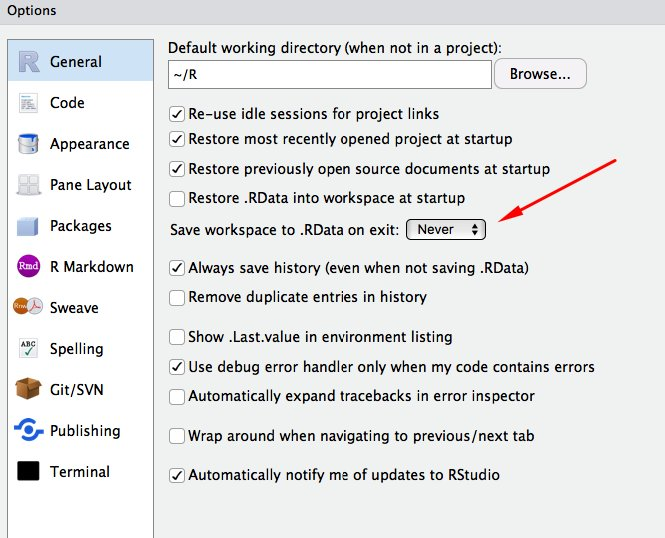
\includegraphics{images/save-workspace-reminder.jpg}
\caption{optional caption text}
\end{figure}

While this may seem like a dramatic step - never saving your workspace -
it is the foundation for doing reproducible work and research using R
Studio (and R). It also represents one of the biggest shifts from using
software like Excel or SPSS, where most steps are not documented in
code. This involves a shift from thinking that your most permanent and
important part of an analysis is your data to thinking of the most
important part as being the code: with the code, you can keep your data
in its original form, process it, and then save a processed file,
through running code. This also means that when you have to make a
change to this code, you can re-run the entire analysis easily.

\subsection{Getting data in and out}\label{getting-data-in-and-out}

\texttt{clipr} is a package to easily copy data into and out of R using
the clipboard. {[}add more{]}

\texttt{datapasta} is another option. {[}add more{]}

\chapter{Education Dataset Analysis Pipeline: Walkthrough
\#1}\label{education-dataset-analysis-pipeline-walkthrough-1}

In the 2015-2016 and 2016-2017 school years, researchers at Michigan
State University carried out a study on students' motivation to learn in
online science classes. The online science classes were part of a
statewide online course provider designed to supplement (and not
replace) students' enrollment in their local school. For example,
students may choose to enroll in an online physics class because one was
not offered at their school (or they were not able to take it given
their schedule).

The study involved a number of different data sources which were brought
to bear to understand students' motivation:

\begin{enumerate}
\def\labelenumi{\arabic{enumi}.}
\tightlist
\item
  A self-report survey for three distinct but related aspects of
  students' motivation
\item
  Log-trace data, such as data output from the learning management
  system
\item
  Achievement-related and gradebook data
\item
  Discussion board data
\item
  Achievement-related (i.e., final grade) data
\end{enumerate}

First, these different data sources will be described in terms of how
they were provided by the school.

\section{1. Self-report survey}\label{self-report-survey}

This was data collected before the start of the course via self-report
survey. The survey included 10 items, each corresponding to one of three
\emph{measures}, namely, for interest, utility value, and perceived
competence:

\begin{enumerate}
\def\labelenumi{\arabic{enumi}.}
\tightlist
\item
  I think this course is an interesting subject. (Interest)
\item
  What I am learning in this class is relevant to my life. (Utility
  value)
\item
  I consider this topic to be one of my best subjects. (Perceive
  competence)
\item
  I am not interested in this course. (Interest - reverse coded)
\item
  I think I will like learning about this topic. (Interest)
\item
  I think what we are studying in this course is useful for me to know.
  (Utility value)
\item
  I don't feel comfortable when it comes to answering questions in this
  area. (Perceived competence)
\item
  I think this subject is interesting. (Interest)
\item
  I find the content of this course to be personally meaningful.
  (Utility value)
\item
  I've always wanted to learn more about this subject. (Interest)
\end{enumerate}

\section{2. Log-trace data}\label{log-trace-data}

Log-trace data is data generated from our interactions with digital
technologies. In education, an increasingly common source of log-trace
data is that generated from interactions with learning management
systems. The data for this walk-through is a \emph{summary of} log-trace
data, namely, the number of minutes students spent on the course. Thus,
while this data is rich, you can imagine even more complex sources of
log-trace data (i.e.~timestamps associated with when students started
and stopped accessing the course!).

\section{3. Achievement-related and gradebook
data}\label{achievement-related-and-gradebook-data}

This is a common source of data, namely, one associated with graded
assignments students completed. In this walkthrough, we just examine
students' final grade.

\section{4. Discussion board data}\label{discussion-board-data}

Discussion board data is both rich and unstructured, in that it is
primarily in the form of written text. We examine a small subset of the
discussion board data in this walkthrough.

\chapter{Processing the data}\label{processing-the-data}

\begin{Shaded}
\begin{Highlighting}[]
\KeywordTok{library}\NormalTok{(readxl)}
\KeywordTok{library}\NormalTok{(tidyverse)}
\KeywordTok{library}\NormalTok{(lubridate)}
\KeywordTok{library}\NormalTok{(here)}
\end{Highlighting}
\end{Shaded}

\begin{Shaded}
\begin{Highlighting}[]
\CommentTok{# Gradebook and log-trace data for F15 and S16 semesters}
\NormalTok{s12_course_data <-}\StringTok{ }\KeywordTok{read_csv}\NormalTok{(}
  \KeywordTok{here}\NormalTok{(}
    \StringTok{"data"}\NormalTok{, }
    \StringTok{"online-science-motivation"}\NormalTok{, }
    \StringTok{"raw"}\NormalTok{, }
    \StringTok{"s12-course-data.csv"}
\NormalTok{  )}
\NormalTok{)}

\CommentTok{# Pre-survey for the F15 and S16 semesters}
\NormalTok{s12_pre_survey  <-}\StringTok{ }\KeywordTok{read_csv}\NormalTok{(}
  \KeywordTok{here}\NormalTok{(}
    \StringTok{"data"}\NormalTok{, }
    \StringTok{"online-science-motivation"}\NormalTok{, }
    \StringTok{"raw"}\NormalTok{, }
    \StringTok{"s12-pre-survey.csv"}
\NormalTok{  )}
\NormalTok{) }

\CommentTok{# Log-trace data for F15 and S16 semesters - ts is for time spent}
\NormalTok{s12_time_spent <-}\StringTok{ }\KeywordTok{read_csv}\NormalTok{(}
  \KeywordTok{here}\NormalTok{(}
    \StringTok{"data"}\NormalTok{, }
    \StringTok{"online-science-motivation"}\NormalTok{, }
    \StringTok{"raw"}\NormalTok{, }
    \StringTok{"s12-course-minutes.csv"}
\NormalTok{  )}
\NormalTok{)}
\end{Highlighting}
\end{Shaded}

\section{Viewing the data}\label{viewing-the-data}

\begin{Shaded}
\begin{Highlighting}[]
\NormalTok{s12_pre_survey }
\NormalTok{s12_course_data}
\NormalTok{s12_time_spent}
\end{Highlighting}
\end{Shaded}

\section{Processing the pre-survey
data}\label{processing-the-pre-survey-data}

Often, survey data needs to be processed in order to be (most) useful.
Here, we process the self-report items into three scales, for: interest,
self-efficacy, and utility value.

\begin{Shaded}
\begin{Highlighting}[]
\CommentTok{# rename the qustions something easier to work with because R is case sensitive}
\CommentTok{# and working with variable names in mix case is prone to error.}

\NormalTok{s12_pre_survey  <-}\StringTok{ }\NormalTok{s12_pre_survey  }\OperatorTok
\StringTok{    }\KeywordTok{rename}\NormalTok{(}\DataTypeTok{q1 =}\NormalTok{ Q1MaincellgroupRow1,}
           \DataTypeTok{q2 =}\NormalTok{ Q1MaincellgroupRow2,}
           \DataTypeTok{q3 =}\NormalTok{ Q1MaincellgroupRow3,}
           \DataTypeTok{q4 =}\NormalTok{ Q1MaincellgroupRow4,}
           \DataTypeTok{q5 =}\NormalTok{ Q1MaincellgroupRow5,}
           \DataTypeTok{q6 =}\NormalTok{ Q1MaincellgroupRow6,}
           \DataTypeTok{q7 =}\NormalTok{ Q1MaincellgroupRow7,}
           \DataTypeTok{q8 =}\NormalTok{ Q1MaincellgroupRow8,}
           \DataTypeTok{q9 =}\NormalTok{ Q1MaincellgroupRow9,}
           \DataTypeTok{q10 =}\NormalTok{ Q1MaincellgroupRow10)}

\CommentTok{# reverse the scale of two questions for consistency.}

\NormalTok{reverse_scale <-}\StringTok{ }\ControlFlowTok{function}\NormalTok{(question) \{}
  \CommentTok{# note, even though 3 is not transformed, case_when expects a match for all}
  \CommentTok{# possible conditions, so it's best practice to label each possible input}
  \CommentTok{# and use TRUE ~ as the final statement returning NA for unexpected inputs.}
\NormalTok{  x <-}\StringTok{ }\KeywordTok{case_when}\NormalTok{(question }\OperatorTok{==}\StringTok{ }\DecValTok{1} \OperatorTok{~}\StringTok{ }\DecValTok{5}
\NormalTok{                 question }\OperatorTok{==}\StringTok{ }\DecValTok{2} \OperatorTok{~}\StringTok{ }\DecValTok{4}\NormalTok{,}
\NormalTok{                 question }\OperatorTok{==}\StringTok{ }\DecValTok{4} \OperatorTok{~}\StringTok{ }\DecValTok{2}\NormalTok{,}
\NormalTok{                 question }\OperatorTok{==}\StringTok{ }\DecValTok{5} \OperatorTok{~}\StringTok{ }\DecValTok{1}\NormalTok{,}
\NormalTok{                 question }\OperatorTok{==}\StringTok{ }\DecValTok{3} \OperatorTok{~}\StringTok{ }\DecValTok{3}\NormalTok{,}
                 \OtherTok{TRUE} \OperatorTok{~}\StringTok{ }\OtherTok{NA_integer_}\NormalTok{)}\ErrorTok{)}
\NormalTok{  x}
\NormalTok{\}}

\NormalTok{s12_pre_survey <-}\StringTok{ }\NormalTok{s12_pre_survey }\OperatorTok
\StringTok{  }\KeywordTok{mutate}\NormalTok{(}\DataTypeTok{q4 =} \KeywordTok{reverse_scale}\NormalTok{(q4),}
         \DataTypeTok{q7 =} \KeywordTok{reverse_scale}\NormalTok{(q7))}

\CommentTok{# Int: 1, 4, 5, 8, 10}
\CommentTok{# UV: 2, 6, 9}
\CommentTok{# PC: 3, 7}

\CommentTok{# need to change these to be within a mutate}
\NormalTok{s12_pre_survey <-}\StringTok{ }\NormalTok{s12_pre_survey }\OperatorTok
\StringTok{  }\KeywordTok{mutate}\NormalTok{(}\DataTypeTok{int =} \KeywordTok{mean}\NormalTok{(q1, q4, q8, q10, q5),}
         \DataTypeTok{uv =} \KeywordTok{mean}\NormalTok{(q2, q6, q9),}
         \DataTypeTok{percomp =} \KeywordTok{mean}\NormalTok{(q3, q7),}
         \DataTypeTok{tv =} \KeywordTok{mean}\NormalTok{(q1, q2, q5, q6, q8, q9, q10)}
\end{Highlighting}
\end{Shaded}

\section{Processing the course data}\label{processing-the-course-data}

We also can process the course data in order to obtain more information.

\begin{Shaded}
\begin{Highlighting}[]
\CommentTok{# split course section into components}
\NormalTok{s12_course_data <-}\StringTok{ }\NormalTok{s12_course_data }\OperatorTok
\StringTok{  }\KeywordTok{separate}\NormalTok{(}\DataTypeTok{col =}\NormalTok{ CourseSectionOrigId,}
           \DataTypeTok{into =} \KeywordTok{c}\NormalTok{(}\StringTok{'subject'}\NormalTok{, }\StringTok{'semester'}\NormalTok{, }\StringTok{'section'}\NormalTok{),}
           \DataTypeTok{sep =} \StringTok{'-'}\NormalTok{,}
           \DataTypeTok{remove =} \OtherTok{FALSE}\NormalTok{)}
\end{Highlighting}
\end{Shaded}

This led to pulling out the subject, semester, and section from the
course ID; variables that we can use later on.

\section{Joining the data}\label{joining-the-data}

To join the course data and pre-survey data, we need to create similar
\emph{keys}. In other words, our goal here is to have one variable that
matches across both datasets, so that we can merge the datasets on the
basis of that variable.

For these data, both have variables for the course and the student,
though they have different names in each. Our first goal will be to
rename two variables in each of our datasets so that they will match.
One variable will correspond to the course, and the other will
correspond to the student. We are not changing anything in the data
itself at this step - instead, we are just cleaning it up so that we can
look at the data all in one place.

Let's start with the pre-survey data. We will rename RespondentID and
opdata\_CourseID to be student\_id and course\_id, respectively.

\begin{Shaded}
\begin{Highlighting}[]
\NormalTok{s12_pre_survey <-}\StringTok{ }\NormalTok{s12_pre_survey }\OperatorTok\StringTok{ }
\StringTok{    }\KeywordTok{rename}\NormalTok{(}\DataTypeTok{student_id =}\NormalTok{ RespondentId,}
           \DataTypeTok{course_id =}\NormalTok{ opdata_CourseID)}

\NormalTok{s12_pre_survey}
\end{Highlighting}
\end{Shaded}

Looks better now!

Let's proceed to the course data. Our goal is to rename two variables
that correspond to the course and the student so that we can match with
the other variables we just created for the pre-survey data.

\begin{Shaded}
\begin{Highlighting}[]
\NormalTok{s12_course_data <-}\StringTok{ }\NormalTok{s12_course_data }\OperatorTok\StringTok{ }
\StringTok{    }\KeywordTok{rename}\NormalTok{(}\DataTypeTok{student_id =}\NormalTok{ Bb_UserPK,}
           \DataTypeTok{course_id =}\NormalTok{ CourseSectionOrigID)}

\NormalTok{s12_course_data}
\end{Highlighting}
\end{Shaded}

Now that we have two variables that are consistent across both datasets
- we have called them ``course\_id'' and ``student\_id'' - we can join
these using the \textbf{dplyr} function, \texttt{left\_join()}. Let's
save our joined data as a new object called ``dat.''

\begin{Shaded}
\begin{Highlighting}[]
\NormalTok{dat <-}\StringTok{ }\KeywordTok{left_join}\NormalTok{(s12_course_data, }
\NormalTok{                 s12_pre_survey, }
                 \DataTypeTok{by =} \KeywordTok{c}\NormalTok{(}\StringTok{"student_id"}\NormalTok{, }\StringTok{"course_id"}\NormalTok{))}

\NormalTok{dat}
\end{Highlighting}
\end{Shaded}

Just one more data frame to merge:

\begin{Shaded}
\begin{Highlighting}[]
\NormalTok{s12_time_spent <-}\StringTok{ }\NormalTok{s12_time_spent }\OperatorTok
\StringTok{  }\KeywordTok{rename}\NormalTok{(}\DataTypeTok{student_id =}\NormalTok{ Bb_UserPK, }
         \DataTypeTok{course_id =}\NormalTok{ CourseSectionOrigID)}
\NormalTok{s12_time_spent <-}\StringTok{ }\NormalTok{s12_time_spent }\OperatorTok
\StringTok{  }\KeywordTok{mutate}\NormalTok{(}\DataTypeTok{student_id =} \KeywordTok{as.integer}\NormalTok{(student_id))}
\NormalTok{dat <-}\StringTok{ }\NormalTok{dat }\OperatorTok\StringTok{ }
\StringTok{  }\KeywordTok{left_join}\NormalTok{(s12_time_spent, }
            \DataTypeTok{by =} \KeywordTok{c}\NormalTok{(}\StringTok{"student_id"}\NormalTok{, }\StringTok{"course_id"}\NormalTok{))}
\end{Highlighting}
\end{Shaded}

Note that they're now combined, even though the course data has many
more rows: The pre\_survey data has been joined for each student by
course combination.

We have a pretty large data frame! Let's take a quick look.

\begin{Shaded}
\begin{Highlighting}[]
\NormalTok{dat}
\end{Highlighting}
\end{Shaded}

It looks like we have neary 30,000 observations from 30 variables.

Now that our data are ready to go, we can start to ask some questions of
the data.

\chapter{Visualizations and Models}\label{visualizations-and-models}

One thing we might be wondering is how time spent on course is related
to students' final grade. Let's first calculate the percentage of points
students earned as a measure of their final grade (noting that the
teacher may have assigned a different grade--or weighted their grades in
ways not reflected through the points).

\begin{Shaded}
\begin{Highlighting}[]
\NormalTok{dat <-}\StringTok{ }\NormalTok{dat }\OperatorTok\StringTok{ }
\StringTok{    }\KeywordTok{group_by}\NormalTok{(student_id, course_id) }\OperatorTok\StringTok{ }
\StringTok{    }\KeywordTok{mutate}\NormalTok{(}\DataTypeTok{Points_Earned =} \KeywordTok{as.integer}\NormalTok{(Points_Earned)) }\OperatorTok\StringTok{ }
\StringTok{    }\KeywordTok{summarize}\NormalTok{(}\DataTypeTok{total_points_possible =} \KeywordTok{sum}\NormalTok{(Points_Possible, }\DataTypeTok{na.rm =} \OtherTok{TRUE}\NormalTok{),}
              \DataTypeTok{total_points_earned =} \KeywordTok{sum}\NormalTok{(Points_Earned, }\DataTypeTok{na.rm =} \OtherTok{TRUE}\NormalTok{)) }\OperatorTok\StringTok{ }
\StringTok{    }\KeywordTok{mutate}\NormalTok{(}\DataTypeTok{percentage_earned =}\NormalTok{ total_points_earned}\OperatorTok{/}\NormalTok{total_points_possible) }\OperatorTok\StringTok{ }
\StringTok{    }\KeywordTok{ungroup}\NormalTok{() }\OperatorTok\StringTok{ }
\StringTok{    }\KeywordTok{left_join}\NormalTok{(dat) }\CommentTok{# note that we join this back to the original data frame to retain all of the variables}
\end{Highlighting}
\end{Shaded}

\section{Visualization of the relationship between time spent on course
and percentage of points
earned}\label{visualization-of-the-relationship-between-time-spent-on-course-and-percentage-of-points-earned}

\begin{Shaded}
\begin{Highlighting}[]
\KeywordTok{ggplot}\NormalTok{(dat, }\KeywordTok{aes}\NormalTok{(}\DataTypeTok{x =}\NormalTok{ TimeSpent, }\DataTypeTok{y =}\NormalTok{ percentage_earned)) }\OperatorTok{+}
\StringTok{    }\KeywordTok{geom_point}\NormalTok{()}
\end{Highlighting}
\end{Shaded}

There appears to be \emph{some} relationship. What if we added a line of
best fit - a linear model?

\begin{Shaded}
\begin{Highlighting}[]
\KeywordTok{ggplot}\NormalTok{(dat, }\KeywordTok{aes}\NormalTok{(}\DataTypeTok{x =}\NormalTok{ TimeSpent, }\DataTypeTok{y =}\NormalTok{ percentage_earned)) }\OperatorTok{+}
\StringTok{    }\KeywordTok{geom_point}\NormalTok{() }\OperatorTok{+}\StringTok{ }
\StringTok{    }\KeywordTok{geom_smooth}\NormalTok{(}\DataTypeTok{method =} \StringTok{"lm"}\NormalTok{)}
\end{Highlighting}
\end{Shaded}

So, it appeares that the more time students spent on the course, the
more points they earned.

\chapter{Linear model (regression)}\label{linear-model-regression}

We can find out exactly what the relationship is using a linear model.

\begin{Shaded}
\begin{Highlighting}[]
\NormalTok{m_linear <-}\StringTok{ }\KeywordTok{lm}\NormalTok{(percentage_earned }\OperatorTok{~}\StringTok{ }\NormalTok{TimeSpent, }\DataTypeTok{data =}\NormalTok{ dat)}
\KeywordTok{summary}\NormalTok{(m_linear)}
\end{Highlighting}
\end{Shaded}

\section{But what about different
courses?}\label{but-what-about-different-courses}

Is there course-specific differences in how much time students spend on
the course as well as in how time spent is related to the percentage of
points students earned?

\begin{Shaded}
\begin{Highlighting}[]
\KeywordTok{ggplot}\NormalTok{(dat, }\KeywordTok{aes}\NormalTok{(}\DataTypeTok{x =}\NormalTok{ TimeSpent, }\DataTypeTok{y =}\NormalTok{ percentage_earned, }\DataTypeTok{color =}\NormalTok{ course_id)) }\OperatorTok{+}
\StringTok{    }\KeywordTok{geom_point}\NormalTok{()}
\end{Highlighting}
\end{Shaded}

\begin{Shaded}
\begin{Highlighting}[]
\KeywordTok{ggplot}\NormalTok{(dat, }\KeywordTok{aes}\NormalTok{(}\DataTypeTok{x =}\NormalTok{ TimeSpent, }\DataTypeTok{y =}\NormalTok{ percentage_earned, }\DataTypeTok{color =}\NormalTok{ course_id)) }\OperatorTok{+}
\StringTok{    }\KeywordTok{geom_point}\NormalTok{() }\OperatorTok{+}
\StringTok{    }\KeywordTok{geom_smooth}\NormalTok{(}\DataTypeTok{method =} \StringTok{"lm"}\NormalTok{)}
\end{Highlighting}
\end{Shaded}

There appears to be so. One way we can test is to use what is called a
multi-level model. This requires a new package; one of the most common
for estimating these types of models is \textbf{lme4}. We use it very
similarly to the \texttt{lm()} function, but we pass it an additional
argument about what the \emph{groups}, or levels, in the data are.

\begin{Shaded}
\begin{Highlighting}[]
\CommentTok{# install.packages("lme4")}
\KeywordTok{library}\NormalTok{(lme4)}
\NormalTok{m_course <-}\StringTok{ }\KeywordTok{lmer}\NormalTok{(percentage_earned }\OperatorTok{~}\StringTok{ }\NormalTok{TimeSpent }\OperatorTok{+}\StringTok{ }\NormalTok{(}\DecValTok{1}\OperatorTok{|}\NormalTok{course_id), }\DataTypeTok{data =}\NormalTok{ dat)}
\KeywordTok{summary}\NormalTok{(m_course)}
\end{Highlighting}
\end{Shaded}

A common way to understand how much variability is at the group level is
to calculate the \emph{intra-class} correlation. This value is the
proportion of the variability in the outcome (the \emph{y}-variable)
that is accounted for solely by the groups identified in the model.
There is a useful function in the \textbf{sjstats} package for doing
this.

\begin{Shaded}
\begin{Highlighting}[]
\CommentTok{# install.packages("sjstats")}
\KeywordTok{library}\NormalTok{(sjstats)}
\KeywordTok{icc}\NormalTok{(m_course)}
\end{Highlighting}
\end{Shaded}

This shows that nearly 17\% of the variability in the percentage of
points students earned can be explained simply by knowing what class
they are in.

\chapter{Education Dataset Analysis Pipeline: Gradebook
Walkthrough}\label{education-dataset-analysis-pipeline-gradebook-walkthrough}

\section{Introduction}\label{introduction-1}

Gradebooks are nearly ubiquitous throughout K-12 classrooms, whether
they exist as standalone Excel files, Google Sheets, or in proprietary
software.

This walkthrough goes through a series of analyses using the data
science framework (link), using the sample
\href{http://web.mit.edu/jabbott/www/excelgradetracker.html}{Assessment
Types - Points} Excel gradebook template from MIT. All data in the
sample gradebook have been generated, and do not reflect individual
student data.

\begin{center}\rule{0.5\linewidth}{\linethickness}\end{center}

\section{Driving Question and
Objectives}\label{driving-question-and-objectives}

\begin{center}\rule{0.5\linewidth}{\linethickness}\end{center}

\section{Data Import}\label{data-import}

Setting up our environment (note: how deep do we go into working
directories?!)

Importing our data (need to sim data for 25 students) Check text for
object naming conventions, discussion of .csv, .xlsx, versatility of
import functions within the \texttt{tidyverse} File naming - issues that
can arise from spaces

\begin{Shaded}
\begin{Highlighting}[]
\NormalTok{gradebook <-}\StringTok{ }\NormalTok{readxl}\OperatorTok{::}\KeywordTok{read_excel}\NormalTok{(}\KeywordTok{here}\NormalTok{(}\StringTok{"/data/gradebooks"}\NormalTok{, }\StringTok{"ExcelGradeTrackerAssessmentTypePoints_SIMDATA_01.xlsx"}\NormalTok{))}
\end{Highlighting}
\end{Shaded}

\section{R Markdown}\label{r-markdown}

This is an R Markdown document. Markdown is a simple formatting syntax
for authoring HTML, PDF, and MS Word documents. For more details on
using R Markdown see \url{http://rmarkdown.rstudio.com}.

When you click the \textbf{Knit} button a document will be generated
that includes both content as well as the output of any embedded R code
chunks within the document. You can embed an R code chunk like this:

\begin{Shaded}
\begin{Highlighting}[]
\KeywordTok{summary}\NormalTok{(cars)}
\end{Highlighting}
\end{Shaded}

\section{Including Plots}\label{including-plots}

You can also embed plots, for example:

Note that the \texttt{echo\ =\ FALSE} parameter was added to the code
chunk to prevent printing of the R code that generated the plot.

\chapter{Education Dataset Analysis Pipeline: Walk Through
\#3}\label{education-dataset-analysis-pipeline-walk-through-3}

\begin{Shaded}
\begin{Highlighting}[]
\CommentTok{# Seed for random number generation}
\KeywordTok{set.seed}\NormalTok{(}\DecValTok{42}\NormalTok{)}
\NormalTok{knitr}\OperatorTok{::}\NormalTok{opts_chunk}\OperatorTok{$}\KeywordTok{set}\NormalTok{(}\DataTypeTok{cache.extra =}\NormalTok{ knitr}\OperatorTok{::}\NormalTok{rand_seed, }\DataTypeTok{eval =} \OtherTok{TRUE}\NormalTok{, }\DataTypeTok{echo =} \OtherTok{FALSE}\NormalTok{, }\DataTypeTok{results =} \StringTok{'hide'}\NormalTok{,}
                      \DataTypeTok{message =} \OtherTok{FALSE}\NormalTok{, }\DataTypeTok{warning =} \OtherTok{FALSE}\NormalTok{)}
\end{Highlighting}
\end{Shaded}

\section{Background}\label{background}

One area of interest is the delivery of online instruction, which is
becoming more prevalent: in 2007, over 3.9 million U.S. students were
enrolled one or more online courses (Allen \& Seaman, 2008).

In this walkthrough, we examine the educational experiences of students
in online science courses at a virtual middle school in order to
characterize their motivation to achieve and their tangible engagement
with the course in terms of behavioral trace measures. To do so, we use
a robust data set, which includes self-reported motivation as well as
behavioral trace data collected from a learning management system (LMS)
to identify predictors of final course grade. Our work examines the idea
of educational success in terms of student interactions with an online
science course.

One meaningful perspective from which to consider students' engagement
with online courses is related to their motivation to achieve. More
specifically, it is important to consider how and why students are
engaging with the course. Considering the psychological mechanisms
behind achievement is valuable because doing so may help to identify
meaningful points of intervention for educators and for researchers and
administrators in online \emph{and} face-to-face courses interested in
the intersection between behavioral trace measures and students'
motivational and affective experiences in such courses.

We take up the following four questions:

\begin{enumerate}
\def\labelenumi{\arabic{enumi}.}
\tightlist
\item
  Is motivation more predictive of course grades as compared to other
  online indicators of engagement?
\item
  Which types of motivation are most predictive of achievement?
\item
  Which types of trace measures are most predictive of achievement?
\item
  How does a random forest compare to a simple linear model
  (regression)?
\end{enumerate}

\section{Information about the
dataset}\label{information-about-the-dataset}

This dataset came from 499 students enrolled in online middle school
science courses in 2015-2016. The data were originally collected for use
as a part of a research study, though the findings have not been
published anywhere, yet.

The setting of this study was a public, provider of individual online
courses in a Midwestern state. In particular, the context was two
semesters (Fall and Spring) of offerings of five online science courses
(Anatomy \& Physiology, Forensic Science, Oceanography, Physics, and
Biology), with a total of 36 classes.

Specific information in the dataset included:

\begin{itemize}
\tightlist
\item
  a pre-course survey students completed about their self-reported
  motivation in science --- in particular, their perceived competence,
  utility value, and interest
\item
  the time students spent on the course (obtained from the LMS,
  Blackboard) and their final course grades as well as their involvement
  in discussion forums
\item
  for discussion board responses, we used the Linguistic Inquiry and
  Word Count (LIWC; Pennebaker, Boyd, Jordan, \& Blackburn, 2015) to
  calculate the number of posts per student and variables for the mean
  levels of students' cognitive processing, positive affect, negative
  affect, and social-related discourse
\end{itemize}

At the beginning of the semester, students were asked to complete the
pre-course survey about their perceived competence, utility value, and
interest. At the end of the semester, the time students spent on the
course, their final course grades, and the contents of the discussion
forums were collected.

In this walkthrough, we used the R package \textbf{caret} to carry out
the analyses.

\section{Information on random
forests}\label{information-on-random-forests}

500 trees were grown as part of our random forest. We partitioned the
data before conducting the main analysis so that neither the training
nor the testing data set would be disproportionately representative of
high-achieving or low-achieving students. The training data set
consisted of 80\% of the original data (n = 400 cases), whereas the
testing data set consisted of 20\% of the original data (n = 99 cases).
We built our random forest model on the training data set, and then
evaluated the model on the testing data set. Three variables were tried
at each node.

Note that the random forest algorithm does not accept cases with missing
data, and so we deleted cases listwise if data were missing. This
decision eliminated 51 cases from our original data set, to bring us to
our final sample size of 499 unique students.

For our analyses, we used Random Forest modeling (Breiman, 2001). Random
forest is an extension of decision tree modeling, whereby a collection
of decision trees are simultaneously ``grown'' and are evaluated based
on out-of-sample predictive accuracy (Breiman, 2001). Random forest is
random in two main ways: first, each tree is only allowed to ``see'' and
split on a limited number of predictors instead of all the predictors in
the parameter space; second, a random subsample of the data is used to
grow each individual tree, such that no individual case is weighted too
heavily in the final prediction.

Whereas some machine learning approaches (e.g., boosted trees) would
utilize an iterative model-building approach, random forest estimates
all the decision trees at once. In this way, each tree is independent of
every other tree. Thus, the random forest algorithm provides a robust
regression approach that is distinct from other modeling approaches. The
final random forest model aggregates the findings across all the
separate trees in the forest in order to offer a collection of ``most
important'' variables as well as a percent variance explained for the
final model.

A random forest is well suited to the research questions that we had
here because it allows for nonlinear modeling. We hypothesized complex
relationships between students' motivation, their engagement with the
online courses, and their achievement. For this reason, a traditional
regressive or structural equation model would have been insufficient to
model the parameter space we were interesting in modeling. Our random
forest model had one outcome and eleven predictors. A common tuning
parameter for machine learning models is the number of variables
considered at each split (Kuhn, 2008); we considered three variables at
each split for this analysis.

The outcome was the final course grade that the student earned. The
predictor variables included motivation variables (interest value,
utility value, and science perceived competence) and trace variables
(the amount of time spent in the course, the course name, the number of
discussion board posts over the course of the semester, the mean level
of cognitive processing evident in discussion board posts, the positive
affect evident in discussion board posts, the negative affect evident in
discussion board posts, and the social-related discourse evident in
their discussion board posts). We used this random forest model to
address all three of our research questions.

To interpret our findings, we examined three main things: (1) predictive
accuracy of the random forest model, (2) variable importance, and (3)
variance explained by the final random forest model.

\section{Analysis}\label{analysis}

\begin{Shaded}
\begin{Highlighting}[]
\KeywordTok{library}\NormalTok{(tidyverse)}
\KeywordTok{library}\NormalTok{(caret)}
\KeywordTok{library}\NormalTok{(here)}
\end{Highlighting}
\end{Shaded}

First, we will load the data, \emph{filter} the data to include only the
data from one year, and \emph{select} variables of interest.

\begin{Shaded}
\begin{Highlighting}[]
\NormalTok{f <-}\StringTok{ }\NormalTok{here}\OperatorTok{::}\KeywordTok{here}\NormalTok{(}\StringTok{"online-science-motivation-w-disc.csv"}\NormalTok{)}

\NormalTok{d <-}\StringTok{ }\KeywordTok{read_csv}\NormalTok{(f)}

\NormalTok{d <-d }\OperatorTok\StringTok{ }\KeywordTok{filter}\NormalTok{(}\OperatorTok{!}\KeywordTok{str_detect}\NormalTok{(course_ID, }\StringTok{"S217"}\NormalTok{))}

\NormalTok{d <-}\StringTok{ }\NormalTok{d }\OperatorTok\StringTok{ }
\StringTok{    }\KeywordTok{select}\NormalTok{(pre_int, pre_uv,  pre_percomp, time_spent,course_ID, final_grade, subject, enrollment_reason, semester, enrollment_status, cogproc, social, posemo, negemo, n)}
\end{Highlighting}
\end{Shaded}

\subsubsection{Use of caret}\label{use-of-caret}

Here, we remove observations with missing data (per our note above about
random forests requiring complete cases).

\begin{Shaded}
\begin{Highlighting}[]
\KeywordTok{nrow}\NormalTok{(d)}
\NormalTok{d <-}\StringTok{ }\KeywordTok{na.omit}\NormalTok{(d)}
\KeywordTok{nrow}\NormalTok{(d)}
\end{Highlighting}
\end{Shaded}

First, machine learning methods often involve using a large number of
variables. Oftentimes, some of these variables will not be suitable to
use: they may be highly correlated with other variables, for instance,
or may have very little - or no - variability. Indeed, for the data set
used in this study, one variables has the same (character string) value
for all of the observations. We can detect this variable and any others
using the following function:

\begin{Shaded}
\begin{Highlighting}[]
\KeywordTok{nearZeroVar}\NormalTok{(d, }\DataTypeTok{saveMetrics =} \OtherTok{TRUE}\NormalTok{)}
\end{Highlighting}
\end{Shaded}

If we look at \texttt{enrollment\_status}, we will see that it is
``Approved/Enrolled'' for \emph{all} of the students. When we use this
in certian models, t may cause some problems, and so we remove it first.

\begin{Shaded}
\begin{Highlighting}[]
\NormalTok{d <-}\StringTok{ }\KeywordTok{select}\NormalTok{(d, }\OperatorTok{-}\NormalTok{enrollment_status)}
\end{Highlighting}
\end{Shaded}

Note that many times you may wish to pre-process the variables, such as
by centering or scaling them; we could this with code like the
following, which is not run here, as we will first try this out with the
variables' original values.

\begin{Shaded}
\begin{Highlighting}[]
\NormalTok{d <-}\StringTok{ }\KeywordTok{mutate_if}\NormalTok{(d, }
\NormalTok{               is.numeric, scale)}
\end{Highlighting}
\end{Shaded}

Now, we will prepare the \textbf{train} and \textbf{test} datasets,
using the caret function for creating data partitions. Here, the
\textbf{p} argument specifies what proportion of the data we want to be
in the \textbf{training} partition. Note that this function splits the
data based upon the outcome, so that the training and test data sets
will both have comparable values for the outcome. Note the
\texttt{times\ =\ 1} argument; this function can be used to create
\emph{multiple} train and test sets, something we will describe in more
detail later.

\begin{Shaded}
\begin{Highlighting}[]
\NormalTok{trainIndex <-}\StringTok{ }\KeywordTok{createDataPartition}\NormalTok{(d}\OperatorTok{$}\NormalTok{final_grade,}
                                  \DataTypeTok{p =}\NormalTok{ .}\DecValTok{8}\NormalTok{, }
                                  \DataTypeTok{list =} \OtherTok{FALSE}\NormalTok{,}
                                  \DataTypeTok{times =} \DecValTok{1}\NormalTok{)}

\NormalTok{d_train <-}\StringTok{ }\NormalTok{d[ trainIndex,] }\CommentTok{# can we make this tidy?}
\NormalTok{d_test <-}\StringTok{ }\NormalTok{d[}\OperatorTok{-}\NormalTok{trainIndex,]}
\end{Highlighting}
\end{Shaded}

Let's turn all of the character variables into factors.

\begin{Shaded}
\begin{Highlighting}[]
\NormalTok{d_test <-}\StringTok{ }\NormalTok{d_test }\OperatorTok
\StringTok{    }\KeywordTok{mutate_if}\NormalTok{(is.character, as.factor)}

\NormalTok{d_train <-}\StringTok{ }\NormalTok{d_train }\OperatorTok
\StringTok{    }\KeywordTok{mutate_if}\NormalTok{(is.character, as.factor)}
\end{Highlighting}
\end{Shaded}

Finally, we will estimate the models.

Here, we will use the train function, passing \emph{all} of the
variables in the data frame (except for the outcome, or dependent
variable, \texttt{final\_grade}) as predictors. NOte that you can read
more about the specific random forest implementation chosen
\href{http://topepo.github.io/caret/train-models-by-tag.html\#random-forest}{here}.

\begin{Shaded}
\begin{Highlighting}[]
\NormalTok{rf_fit <-}\StringTok{ }\KeywordTok{train}\NormalTok{(final_grade }\OperatorTok{~}\StringTok{ }\NormalTok{.,}
                \DataTypeTok{data =}\NormalTok{ d_train,}
                \DataTypeTok{method =} \StringTok{"ranger"}\NormalTok{)}

\NormalTok{rf_fit}
\end{Highlighting}
\end{Shaded}

We have some results! First, we see that we have 400 samples, or 400
observations, the number in the train data set. No pre-processing steps
were specified in the model fitting (note that) these the output of
\texttt{preProcess} can be passed to \texttt{train()} to center, scale,
and transform the data in many other ways. Next, note that a resampling
technique has been used: this is not for validating the model (per se),
but is rather for selecting tuning parameters, or options that need to
be specified as a part of the modeling. These parameters can be manually
provided, or can be estimated via strategies such as the bootstrap
resample (or \emph{k}-folds cross validation).

It appears that the model with the value of the \textbf{mtry} tuning
parameter equal to 42 seemed to explain the data best, the
\textbf{splirule* being ``extratrees'', and }min.node.size** held
constant at a value of 5.

Let's see if we end up with slightly different values if we change the
resampling technique to cross-validation, instead of bootstrap
resampling.

\begin{Shaded}
\begin{Highlighting}[]
\NormalTok{train_control <-}\StringTok{ }\KeywordTok{trainControl}\NormalTok{(}\DataTypeTok{method =} \StringTok{"repeatedcv"}\NormalTok{,}
                              \DataTypeTok{number =} \DecValTok{10}\NormalTok{,}
                              \DataTypeTok{repeats =} \DecValTok{10}\NormalTok{)}

\NormalTok{rf_fit1 <-}\StringTok{ }\KeywordTok{train}\NormalTok{(final_grade }\OperatorTok{~}\StringTok{ }\NormalTok{.,}
                \DataTypeTok{data =}\NormalTok{ d_train,}
                \DataTypeTok{method =} \StringTok{"ranger"}\NormalTok{,}
                \DataTypeTok{trControl =}\NormalTok{ train_control)}

\NormalTok{rf_fit1}
\end{Highlighting}
\end{Shaded}

The same tuning parameter values seem to be found with this method.
Let's check just one last thing - what if we do not fix
\textbf{min.node.size} to five?

Let's create our own grid of values to test. We'll stick with the
default bootstrap resampling method to choose the best model.

\begin{Shaded}
\begin{Highlighting}[]
\NormalTok{tune_grid <-}\StringTok{ }\KeywordTok{expand.grid}\NormalTok{(}\DataTypeTok{mtry =} \KeywordTok{c}\NormalTok{(}\DecValTok{2}\NormalTok{, }\DecValTok{22}\NormalTok{, }\DecValTok{42}\NormalTok{),}
                         \DataTypeTok{splitrule =} \KeywordTok{c}\NormalTok{(}\StringTok{"variance"}\NormalTok{, }\StringTok{"extratrees"}\NormalTok{),}
                         \DataTypeTok{min.node.size =} \KeywordTok{c}\NormalTok{(}\DecValTok{1}\NormalTok{, }\DecValTok{5}\NormalTok{, }\DecValTok{10}\NormalTok{, }\DecValTok{15}\NormalTok{, }\DecValTok{20}\NormalTok{))}

\NormalTok{rf_fit2 <-}\StringTok{ }\KeywordTok{train}\NormalTok{(final_grade }\OperatorTok{~}\StringTok{ }\NormalTok{.,}
                \DataTypeTok{data =}\NormalTok{ d_train,}
                \DataTypeTok{method =} \StringTok{"ranger"}\NormalTok{,}
                \DataTypeTok{tuneGrid =}\NormalTok{ tune_grid)}

\NormalTok{rf_fit2}
\end{Highlighting}
\end{Shaded}

The model with the same values as identified before but with
\textbf{min.node.size} equal to 1 seems to fit best, though the
improvement seems to be fairly small relative to the difference the
other tuning parameters seem to make.

Let's take a look at this model. We will first note the large number of
independent variables: this is due to the factors being treated as dummy
codes. We can also note the *OOB prediction error (MSE)`, of 0.351, and
the proportion of the variance explained, or R squared, of 0.658.

\begin{Shaded}
\begin{Highlighting}[]
\NormalTok{rf_fit2}\OperatorTok{$}\NormalTok{finalModel}
\end{Highlighting}
\end{Shaded}

Things to do next\ldots{}

\begin{itemize}
\tightlist
\item
  see how predicted values compare to those in the test set to
  understand predictive accuracy
\item
  examine variable importance
\item
  compare predictive accuracy of the model to a linear model
  (regression)
\end{itemize}

\chapter{Education Dataset Analysis Pipeline: Walk Through
\#4}\label{education-dataset-analysis-pipeline-walk-through-4}

\section{Background}\label{background-1}

Relationships are important to us. In the case of many research
techniques, relationships are--deservedly--the focus of analyses. It is
not very difficult to imagine \emph{qualitative} techniques to study
relationships: One could ask other individuals about who their friends
are, why they are their friends, and what they like to do when with
them.

Increasingly, it is also not hard to imagine \emph{quantitative}
techniques to study relationships, too. In a way, the same questions
that could be used qualitatively can serve as the basis for the
quantitative study of relationships. Indeed, social network analysis
uses these relations in a range of visualizations as well as statistical
models.

Let us first consider visualizations.

Visualizations of social networks are interesting and powerful--and
increasingly common.

Behind these visualizations, though, there are also statistical models
and methods that can help to understand what is going on with respect to
particular relationships in a network in additional ways.

\section{Selection and influence}\label{selection-and-influence}

One way to consider these models and methods is in terms of two
\emph{processes} at play in our relationships (cite). These two
processes are commonly (though not exclusively) the focus of statistical
analyses of networks. In addition to not being exclusive, they do not
interact independently: they affect each other reciprocally (Xu, Frank,
\& Penuel, 2018). They are:

\begin{itemize}
\tightlist
\item
  Selection: the processes regarding who chooses to have a relationship
  with whom
\item
  Infuence: the processes regarding how who we have relationships with
  affects our behavior
\end{itemize}

While these are complex, they can be studied with the type of data
collected from asking people about their relationships (and possibly
asking them about or studying their behavior--or measuring some
outcome). Happily, the use of these methods has expanded along with
\textbf{R}: many of the best tools for studying social networks are in
the form of long-standing R packages. Additionally, while there are many
potential naunces to studying selection and influence, these are models
that can fundamentally be carried out with regression, or the linear
model (or extensions of it)

In this walkthrough, the influence model is the focus. Nevertheless, we
provide some direction for how to carry out selection modeling, too, at
the end.

\section{An example of influence}\label{an-example-of-influence}

In this example, we create some example data that can be used to explore
questions about how influence works. Note that Joshua Rosenberg and
Sarah Galey initially wrote the following code for a walkthrough shared
on Ken Frank's website
\href{https://msu.edu/~kenfrank/resources.htm}{here}.

\subsection{Creating example data in the form of an
edgelist}\label{creating-example-data-in-the-form-of-an-edgelist}

First, let's create three different data frames. Here is what they
should contain:

\begin{itemize}
\tightlist
\item
  A data frame indicating who the \emph{nominator} and \emph{nominee}
  for the relation (i.e., if Stefanie says that José is her friend, then
  Stefanie is the nominator and José the nominee) - as well as an
  optional variable indicating the weight, or strength, of their
  relation

  \begin{itemize}
  \tightlist
  \item
    This data frame and its type can be considered the basis for many
    types of social network analysis and is a common structure for
    network data: it is an \emph{edgelist}
  \end{itemize}
\item
  Data frames indicating the values of some behavior - an outcome - at
  two different time points
\end{itemize}

We use the \textbf{simstudy} package to simulate the data (and the
\textbf{dplyr} package to process the data a bit).

Let's first generate \texttt{data1}.

\begin{Shaded}
\begin{Highlighting}[]
\KeywordTok{library}\NormalTok{(simstudy)}
\KeywordTok{library}\NormalTok{(dplyr)}

\KeywordTok{set.seed}\NormalTok{(}\StringTok{"20190101"}\NormalTok{)}

\NormalTok{def <-}\StringTok{ }\KeywordTok{defData}\NormalTok{(}\DataTypeTok{varname =} \StringTok{"nominator"}\NormalTok{, }\DataTypeTok{dist =} \StringTok{"categorical"}\NormalTok{, }\DataTypeTok{formula =} \KeywordTok{catProbs}\NormalTok{(}\DataTypeTok{n =} \DecValTok{200}\NormalTok{)) }
\NormalTok{def <-}\StringTok{ }\KeywordTok{defData}\NormalTok{(def, }\DataTypeTok{varname =} \StringTok{"nominee"}\NormalTok{, }\DataTypeTok{dist =} \StringTok{"categorical"}\NormalTok{, }\DataTypeTok{formula =} \KeywordTok{catProbs}\NormalTok{(}\DataTypeTok{n =} \DecValTok{200}\NormalTok{))}
\NormalTok{def <-}\StringTok{ }\KeywordTok{defData}\NormalTok{(def, }\DataTypeTok{varname =} \StringTok{"relate"}\NormalTok{, }\DataTypeTok{dist =} \StringTok{"nonrandom"}\NormalTok{, }\DataTypeTok{formula =} \DecValTok{1}\NormalTok{)}

\NormalTok{data1 <-}\StringTok{ }\KeywordTok{genData}\NormalTok{(}\DecValTok{500}\NormalTok{, def)}
\end{Highlighting}
\end{Shaded}

\texttt{data2}:

\begin{Shaded}
\begin{Highlighting}[]
\NormalTok{unique_nominators <-}\StringTok{ }\KeywordTok{unique}\NormalTok{(data1}\OperatorTok{$}\NormalTok{nominator) }\CommentTok{# need these to determine how many rows to generate}
\NormalTok{unique_nominees <-}\StringTok{ }\KeywordTok{unique}\NormalTok{(data1}\OperatorTok{$}\NormalTok{nominee)}

\NormalTok{def <-}\StringTok{ }\KeywordTok{defData}\NormalTok{(}\DataTypeTok{varname =} \StringTok{"yvar1"}\NormalTok{, }\DataTypeTok{dist =} \StringTok{"normal"}\NormalTok{, }\DataTypeTok{formula =} \DecValTok{2}\NormalTok{, }\DataTypeTok{variance =} \DecValTok{2}\NormalTok{)}

\NormalTok{data2 <-}\StringTok{ }\KeywordTok{genData}\NormalTok{(}\KeywordTok{length}\NormalTok{(unique_nominees), def)}
\NormalTok{data2 <-}\StringTok{ }\NormalTok{data2 }\OperatorTok\StringTok{ }
\StringTok{    }\KeywordTok{mutate}\NormalTok{(}\DataTypeTok{nominee =}\NormalTok{ unique_nominees) }\OperatorTok\StringTok{ }
\StringTok{    }\KeywordTok{select}\NormalTok{(nominee, yvar1)}
\end{Highlighting}
\end{Shaded}

And \texttt{data3}:

\begin{Shaded}
\begin{Highlighting}[]
\NormalTok{def <-}\StringTok{ }\KeywordTok{defData}\NormalTok{(}\DataTypeTok{varname =} \StringTok{"yvar2"}\NormalTok{, }\DataTypeTok{dist =} \StringTok{"normal"}\NormalTok{, }\DataTypeTok{formula =} \DecValTok{5}\NormalTok{, }\DataTypeTok{variance =} \DecValTok{2}\NormalTok{)}

\NormalTok{data3 <-}\StringTok{ }\KeywordTok{genData}\NormalTok{(}\KeywordTok{length}\NormalTok{(unique_nominators), def)}
\NormalTok{data3 <-}\StringTok{ }\NormalTok{data3 }\OperatorTok\StringTok{ }
\StringTok{    }\KeywordTok{mutate}\NormalTok{(}\DataTypeTok{nominator =}\NormalTok{ unique_nominees) }\OperatorTok\StringTok{ }
\StringTok{    }\KeywordTok{select}\NormalTok{(nominator, yvar2)}
\end{Highlighting}
\end{Shaded}

\subsection{Joining the data}\label{joining-the-data-1}

Next, we'll join the data into one data frame. Note that while this is
sometimes tedius and time-consuming, especially with large sources of
network data, it is a key step for being able to carry out network
analysis - often, even for creating visualiations that are informative.

\begin{Shaded}
\begin{Highlighting}[]
\KeywordTok{library}\NormalTok{(dplyr)}

\NormalTok{data <-}\StringTok{ }\KeywordTok{left_join}\NormalTok{(data1, data2, }\DataTypeTok{by =} \StringTok{"nominee"}\NormalTok{)}
\NormalTok{data}\OperatorTok{$}\NormalTok{nominee <-}\StringTok{ }\KeywordTok{as.character}\NormalTok{(data}\OperatorTok{$}\NormalTok{nominee) }\CommentTok{# this makes merging later easier}

\CommentTok{# calculate indegree in tempdata and merge with data}
\NormalTok{tempdata <-}\StringTok{ }\KeywordTok{data.frame}\NormalTok{(}\KeywordTok{table}\NormalTok{(data}\OperatorTok{$}\NormalTok{nominee)) }\CommentTok{# this needs to be calculated differently}
\KeywordTok{names}\NormalTok{(tempdata) <-}\StringTok{ }\KeywordTok{c}\NormalTok{(}\StringTok{"nominee"}\NormalTok{, }\StringTok{"indegree"}\NormalTok{) }\CommentTok{# rename the column "nominee"}
\NormalTok{tempdata}\OperatorTok{$}\NormalTok{nominee <-}\StringTok{ }\KeywordTok{as.character}\NormalTok{(tempdata}\OperatorTok{$}\NormalTok{nominee) }\CommentTok{# makes nominee a character data type, instead of a factor, which can cause problems}
\NormalTok{data <-}\StringTok{ }\KeywordTok{left_join}\NormalTok{(data, tempdata, }\DataTypeTok{by =} \StringTok{"nominee"}\NormalTok{)}
\end{Highlighting}
\end{Shaded}

Let's take a look at the merged data.

\begin{Shaded}
\begin{Highlighting}[]
\NormalTok{data <-}\StringTok{ }\KeywordTok{as_tibble}\NormalTok{(data)}
\NormalTok{data}
\end{Highlighting}
\end{Shaded}

\subsection{Calculating an exposure
term}\label{calculating-an-exposure-term}

This is the key step that makes this model - a regression, or linear,
model - one that is special. It is creating an exposure term. The idea
is that the exposure term ``captures'' how your interactions with
someone, over some period of time (between the first and second time
points) impact some outcome. This model accounts for an individual's
initial report of the outcome, i.e., their time 1 prior value, so it is
a model for \emph{change} in some outcome.

\begin{Shaded}
\begin{Highlighting}[]
\CommentTok{# Calculating exposure}
\NormalTok{data}\OperatorTok{$}\NormalTok{exposure <-}\StringTok{ }\NormalTok{data}\OperatorTok{$}\NormalTok{relate }\OperatorTok{*}\StringTok{ }\NormalTok{data}\OperatorTok{$}\NormalTok{yvar1}

\CommentTok{# Calculating mean exposure}
\NormalTok{mean_exposure <-}\StringTok{ }\NormalTok{data }\OperatorTok
\StringTok{    }\KeywordTok{group_by}\NormalTok{(nominator) }\OperatorTok
\StringTok{    }\KeywordTok{summarize}\NormalTok{(}\DataTypeTok{exposure_mean =} \KeywordTok{mean}\NormalTok{(exposure))}
\end{Highlighting}
\end{Shaded}

What this data frame - \texttt{mean\_exposure} - contains is the mean of
the outcome (in this case, \texttt{yvar1}) for all of the individuals
the nominator had a relation with.

As we need a final data set with \texttt{mean\_exposure},
\texttt{mean\_exposure\_plus}, \texttt{degree}, \texttt{yvar1}, and
\texttt{yvar2} added, we'll process the data a bit more.

\begin{Shaded}
\begin{Highlighting}[]
\NormalTok{mean_exposure_terms <-}\StringTok{ }\KeywordTok{left_join}\NormalTok{(mean_exposure, mean_exposure_plus, }\DataTypeTok{by =} \StringTok{"nominator"}\NormalTok{)}

\KeywordTok{names}\NormalTok{(data2) <-}\StringTok{ }\KeywordTok{c}\NormalTok{(}\StringTok{"nominator"}\NormalTok{, }\StringTok{"yvar1"}\NormalTok{) }\CommentTok{# rename nominee as nominator to merge these}
\NormalTok{final_data <-}\StringTok{ }\KeywordTok{left_join}\NormalTok{(mean_exposure_terms, data2, }\DataTypeTok{by =} \StringTok{"nominator"}\NormalTok{)}
\NormalTok{final_data <-}\StringTok{ }\KeywordTok{left_join}\NormalTok{(final_data, data3, }\DataTypeTok{by =} \StringTok{"nominator"}\NormalTok{) }\CommentTok{# data3 already has nominator, so no need to change}
\end{Highlighting}
\end{Shaded}

\subsection{Regression (linear models)}\label{regression-linear-models}

Calculating the exposure term is the most distinctive and important step
in carrying out influence models. Now, we can simply use a linear model
to find out how much relations - as captured by the influence term -
affect some outcome.

\begin{Shaded}
\begin{Highlighting}[]
\NormalTok{model1 <-}\StringTok{ }\KeywordTok{lm}\NormalTok{(yvar2 }\OperatorTok{~}\StringTok{ }\NormalTok{yvar1 }\OperatorTok{+}\StringTok{ }\NormalTok{exposure_mean, }\DataTypeTok{data =}\NormalTok{ final_data)}
\KeywordTok{summary}\NormalTok{(model1)}
\end{Highlighting}
\end{Shaded}

Note that these models show \ldots{}

So, the influence model is used to study a key process for social
network analysis, but it is one that is useful, because you can
quantify, given what you measure and how you measure it, \emph{the
network effect}, something that is sometimes not considered, especially
in education (Sweet, 2017). It's also fundamentally a regression. That's
really it, as the majority of the work goes into calculating the
exposure term.

\section{Selection models}\label{selection-models}

While this tutorial focused on influence models, selection models are
also commonly used - and are commonly of interest not only to
researchers but also to administrators and teachers (and even to youth
and students).

Here, we briefly describe a few possible approaches for using a
selection model.

At its core, the selection model is a regression - albeit, one that is a
generalization of one, namely, a logistic regression (sometimes termed a
generalized linear model, because it is \emph{basically} a regression
but is one with an outcome that consists just of 0's and 1's). Thus, the
most straight-away way to use a selection model is to use a logistic
regression where all of the relations (note the \texttt{relate} variable
in \texttt{data1} above) are indicated with a 1. But, here is the
important and challenging step: all of the \emph{possible relations}
(i.e., all of the relations that are possible between all of the
individuals in a network) are indicated with a 0 in an edgelist. Note
that, again, an edgelist is the preferred data structure for carrying
out this analysis. This step involves some data wrangling, especially
the idea of widening or lengthening a data frame.

Once all of the relations are indicated with a 1 or a 0, then a simple
linear regression can be used. Imagine that we are interested in whether
individuals from the \emph{same} group are more or less likely to
interact than those from different groups; same could be created in the
data frame based upon knowing which group both nominator and nominee are
from:

\begin{Shaded}
\begin{Highlighting}[]
\NormalTok{m_selection <-}\StringTok{ }\KeywordTok{glm}\NormalTok{(relate }\OperatorTok{~}\StringTok{ }\DecValTok{1} \OperatorTok{+}\StringTok{ }\NormalTok{same, }\DataTypeTok{data =}\NormalTok{ edgelist1)}
\end{Highlighting}
\end{Shaded}

While this is a straightforward way to carry out a selection model,
there are some limitations to it. Namely, it does not account for
individuals who send more (or less) nominations overall--and not
considering this may mean other effects, like the one associated with
being from the \emph{same} group, are not accurate. A few extensions of
the linear model - including those that can use data for which
relationships are indicated with weights, not just 1's and 0's, have
been developed.

One type of model extends the logistic regression. It can be used for
data that is not only 1's and 0's but also data that is normally
distributed or has fixed-ranks. It is the \textbf{amen} package
available
\href{https://cran.r-project.org/web/packages/amen/index.html}{here}.

A particularly common one is an Exponential Random Graph Model, or an
ERGM. An R package that makes estimating these easy is available
\href{https://cran.r-project.org/web/packages/ergm/index.html}{here}.
That R package, \textbf{ergm}, is part of a powerful and often-used
collection of packages, including those for working with network data
(data that can begin with an edgelist, but may need additional
processing that is challenging to do with edgelist data),
\textbf{statnet}. A link to the statnet packages is
\href{https://statnet.org/}{here}.

\chapter{Advanced Uses}\label{advanced-uses}

\section{Multi-level models}\label{multi-level-models}

This is an example from the online science motivation dataset.

\begin{Shaded}
\begin{Highlighting}[]
\NormalTok{d <-}\StringTok{ }\NormalTok{readr}\OperatorTok{::}\KeywordTok{read_csv}\NormalTok{(}\StringTok{"data/online-science-motivation.csv"}\NormalTok{)}
\NormalTok{d}
\end{Highlighting}
\end{Shaded}

\section{Text analysis}\label{text-analysis}

\section{Longitudinal analysis}\label{longitudinal-analysis}

\chapter{Solutions for Adopting Data Science Techniques in
Education}\label{solutions-for-adopting-data-science-techniques-in-education}

\chapter{Students doing data science}\label{students-doing-data-science}

\chapter{Resources used in the creation of this
text}\label{resources-used-in-the-creation-of-this-text}

\textbf{\href{http://ncrpp.org/assets/documents/NCRPP_Technical-Report-1_National-Survey-of-Research-Use.pdf}{National
Center for Research in Policy and Practice: Findings from a National
Study on Research Use Among School and District Leaders}}

\emph{Summary}: A survey of 733 school principals and district leaders
within US mid-sized and large school districts, focused on how
educational leaders use research to inform their decision-making.


\end{document}
